% Options for packages loaded elsewhere
\PassOptionsToPackage{unicode}{hyperref}
\PassOptionsToPackage{hyphens}{url}
%
\documentclass[
]{article}
\usepackage{amsmath,amssymb}
\usepackage{lmodern}
\usepackage{ifxetex,ifluatex}
\ifnum 0\ifxetex 1\fi\ifluatex 1\fi=0 % if pdftex
  \usepackage[T1]{fontenc}
  \usepackage[utf8]{inputenc}
  \usepackage{textcomp} % provide euro and other symbols
\else % if luatex or xetex
  \usepackage{unicode-math}
  \defaultfontfeatures{Scale=MatchLowercase}
  \defaultfontfeatures[\rmfamily]{Ligatures=TeX,Scale=1}
\fi
% Use upquote if available, for straight quotes in verbatim environments
\IfFileExists{upquote.sty}{\usepackage{upquote}}{}
\IfFileExists{microtype.sty}{% use microtype if available
  \usepackage[]{microtype}
  \UseMicrotypeSet[protrusion]{basicmath} % disable protrusion for tt fonts
}{}
\makeatletter
\@ifundefined{KOMAClassName}{% if non-KOMA class
  \IfFileExists{parskip.sty}{%
    \usepackage{parskip}
  }{% else
    \setlength{\parindent}{0pt}
    \setlength{\parskip}{6pt plus 2pt minus 1pt}}
}{% if KOMA class
  \KOMAoptions{parskip=half}}
\makeatother
\usepackage{xcolor}
\IfFileExists{xurl.sty}{\usepackage{xurl}}{} % add URL line breaks if available
\IfFileExists{bookmark.sty}{\usepackage{bookmark}}{\usepackage{hyperref}}
\hypersetup{
  pdftitle={Quelques notes sur les statistiques},
  pdfauthor={P.Gaignon},
  hidelinks,
  pdfcreator={LaTeX via pandoc}}
\urlstyle{same} % disable monospaced font for URLs
\usepackage[margin=1in]{geometry}
\usepackage{color}
\usepackage{fancyvrb}
\newcommand{\VerbBar}{|}
\newcommand{\VERB}{\Verb[commandchars=\\\{\}]}
\DefineVerbatimEnvironment{Highlighting}{Verbatim}{commandchars=\\\{\}}
% Add ',fontsize=\small' for more characters per line
\usepackage{framed}
\definecolor{shadecolor}{RGB}{248,248,248}
\newenvironment{Shaded}{\begin{snugshade}}{\end{snugshade}}
\newcommand{\AlertTok}[1]{\textcolor[rgb]{0.94,0.16,0.16}{#1}}
\newcommand{\AnnotationTok}[1]{\textcolor[rgb]{0.56,0.35,0.01}{\textbf{\textit{#1}}}}
\newcommand{\AttributeTok}[1]{\textcolor[rgb]{0.77,0.63,0.00}{#1}}
\newcommand{\BaseNTok}[1]{\textcolor[rgb]{0.00,0.00,0.81}{#1}}
\newcommand{\BuiltInTok}[1]{#1}
\newcommand{\CharTok}[1]{\textcolor[rgb]{0.31,0.60,0.02}{#1}}
\newcommand{\CommentTok}[1]{\textcolor[rgb]{0.56,0.35,0.01}{\textit{#1}}}
\newcommand{\CommentVarTok}[1]{\textcolor[rgb]{0.56,0.35,0.01}{\textbf{\textit{#1}}}}
\newcommand{\ConstantTok}[1]{\textcolor[rgb]{0.00,0.00,0.00}{#1}}
\newcommand{\ControlFlowTok}[1]{\textcolor[rgb]{0.13,0.29,0.53}{\textbf{#1}}}
\newcommand{\DataTypeTok}[1]{\textcolor[rgb]{0.13,0.29,0.53}{#1}}
\newcommand{\DecValTok}[1]{\textcolor[rgb]{0.00,0.00,0.81}{#1}}
\newcommand{\DocumentationTok}[1]{\textcolor[rgb]{0.56,0.35,0.01}{\textbf{\textit{#1}}}}
\newcommand{\ErrorTok}[1]{\textcolor[rgb]{0.64,0.00,0.00}{\textbf{#1}}}
\newcommand{\ExtensionTok}[1]{#1}
\newcommand{\FloatTok}[1]{\textcolor[rgb]{0.00,0.00,0.81}{#1}}
\newcommand{\FunctionTok}[1]{\textcolor[rgb]{0.00,0.00,0.00}{#1}}
\newcommand{\ImportTok}[1]{#1}
\newcommand{\InformationTok}[1]{\textcolor[rgb]{0.56,0.35,0.01}{\textbf{\textit{#1}}}}
\newcommand{\KeywordTok}[1]{\textcolor[rgb]{0.13,0.29,0.53}{\textbf{#1}}}
\newcommand{\NormalTok}[1]{#1}
\newcommand{\OperatorTok}[1]{\textcolor[rgb]{0.81,0.36,0.00}{\textbf{#1}}}
\newcommand{\OtherTok}[1]{\textcolor[rgb]{0.56,0.35,0.01}{#1}}
\newcommand{\PreprocessorTok}[1]{\textcolor[rgb]{0.56,0.35,0.01}{\textit{#1}}}
\newcommand{\RegionMarkerTok}[1]{#1}
\newcommand{\SpecialCharTok}[1]{\textcolor[rgb]{0.00,0.00,0.00}{#1}}
\newcommand{\SpecialStringTok}[1]{\textcolor[rgb]{0.31,0.60,0.02}{#1}}
\newcommand{\StringTok}[1]{\textcolor[rgb]{0.31,0.60,0.02}{#1}}
\newcommand{\VariableTok}[1]{\textcolor[rgb]{0.00,0.00,0.00}{#1}}
\newcommand{\VerbatimStringTok}[1]{\textcolor[rgb]{0.31,0.60,0.02}{#1}}
\newcommand{\WarningTok}[1]{\textcolor[rgb]{0.56,0.35,0.01}{\textbf{\textit{#1}}}}
\usepackage{longtable,booktabs,array}
\usepackage{calc} % for calculating minipage widths
% Correct order of tables after \paragraph or \subparagraph
\usepackage{etoolbox}
\makeatletter
\patchcmd\longtable{\par}{\if@noskipsec\mbox{}\fi\par}{}{}
\makeatother
% Allow footnotes in longtable head/foot
\IfFileExists{footnotehyper.sty}{\usepackage{footnotehyper}}{\usepackage{footnote}}
\makesavenoteenv{longtable}
\usepackage{graphicx}
\makeatletter
\def\maxwidth{\ifdim\Gin@nat@width>\linewidth\linewidth\else\Gin@nat@width\fi}
\def\maxheight{\ifdim\Gin@nat@height>\textheight\textheight\else\Gin@nat@height\fi}
\makeatother
% Scale images if necessary, so that they will not overflow the page
% margins by default, and it is still possible to overwrite the defaults
% using explicit options in \includegraphics[width, height, ...]{}
\setkeys{Gin}{width=\maxwidth,height=\maxheight,keepaspectratio}
% Set default figure placement to htbp
\makeatletter
\def\fps@figure{htbp}
\makeatother
\setlength{\emergencystretch}{3em} % prevent overfull lines
\providecommand{\tightlist}{%
  \setlength{\itemsep}{0pt}\setlength{\parskip}{0pt}}
\setcounter{secnumdepth}{5}
\usepackage{ucs}
\usepackage[T1]{fontenc}
\newcommand*\chancery{\fontfamily{pzc}\selectfont}
\usepackage{float}
\floatplacement{figure}{H}
\usepackage{tgschola}
\usepackage{frcursive}
\usepackage{latexsym,amsmath,amssymb,textcomp,amsfonts}
\usepackage{graphicx}
\usepackage{nccpic}
\usepackage{setspace}
\usepackage{multicol}
\usepackage{url}
\usepackage{wrapfig}
\usepackage{setspace}
\linespread{1.5}
\usepackage{hyperref}
\usepackage{geometry}
\usepackage{tikz}
\usetikzlibrary{snakes}
\usepackage{tcolorbox}
\renewcommand{\thesection}{\Roman{section})}
\renewcommand{\thesubsection}{\alph{subsection}}
\usepackage{titlesec}
\titlespacing{\section}{0cm}{1cm}{0.4cm}
\titlespacing{\subsection}{0.7cm}{0.2cm}{0.1cm}
\titlespacing{\subsubsection}{1.4cm}{0.cm}{0.1cm}
\titlespacing{\paragraph}{2.1cm}{0.cm}{0.1cm}
\usepackage{tocloft}
\addtolength{\cftsecnumwidth}{10pt}
\usepackage{chngcntr}
\counterwithin{figure}{section}
\makeatletter
\renewcommand*\l@figure{\@dottedtocline{1}{1em}{3.2em}}
\makeatother
\usepackage{booktabs}
\usepackage{longtable}
\usepackage{array}
\usepackage{multirow}
\usepackage{wrapfig}
\usepackage{float}
\usepackage{colortbl}
\usepackage{pdflscape}
\usepackage{tabu}
\usepackage{threeparttable}
\usepackage{threeparttablex}
\usepackage[normalem]{ulem}
\usepackage{makecell}
\usepackage{xcolor}
\ifluatex
  \usepackage{selnolig}  % disable illegal ligatures
\fi
\newlength{\cslhangindent}
\setlength{\cslhangindent}{1.5em}
\newlength{\csllabelwidth}
\setlength{\csllabelwidth}{3em}
\newenvironment{CSLReferences}[2] % #1 hanging-ident, #2 entry spacing
 {% don't indent paragraphs
  \setlength{\parindent}{0pt}
  % turn on hanging indent if param 1 is 1
  \ifodd #1 \everypar{\setlength{\hangindent}{\cslhangindent}}\ignorespaces\fi
  % set entry spacing
  \ifnum #2 > 0
  \setlength{\parskip}{#2\baselineskip}
  \fi
 }%
 {}
\usepackage{calc}
\newcommand{\CSLBlock}[1]{#1\hfill\break}
\newcommand{\CSLLeftMargin}[1]{\parbox[t]{\csllabelwidth}{#1}}
\newcommand{\CSLRightInline}[1]{\parbox[t]{\linewidth - \csllabelwidth}{#1}\break}
\newcommand{\CSLIndent}[1]{\hspace{\cslhangindent}#1}

\title{Quelques notes sur les statistiques}
\author{P.Gaignon}
\date{\today}

\begin{document}
\maketitle

{
\setcounter{tocdepth}{4}
\tableofcontents
}
\pagebreak

\listoffigures

\section*{A propos de ce document :}

Ce document est destiné à une utilisation non commerciale. Le but est
juste de partager les connaissances que j'ai pu acquises en statistiques
aux travers de mon expérience. L'objectif n'est pas de faire un document
de référence / cours, mais un partage d'expérience. J'essaye autant que
possible d'ajouter les références des données et références utilisés.

Pour chaque partie, il est précisé les packages nécessaires à installer
pour faire tourner le code proposé. Il est également important
d'installer les dépendances des packages pour que tout fonctionne. Des
commentaires de code sont également ajoutés pour expliquer certains
éléments particuliers lors de la mise en pratique sous R.

Attention, il ne s'agit pas d'un document apprenant à coder en R, mais
donnant les éléments nécessaires pour réaliser certaines analyses. La
majorité des analyses sont réalisées à partir de données déjà présentes
dans R.

\pagebreak

\hypertarget{quelques-bases-statistiques}{%
\section{Quelques bases
statistiques}\label{quelques-bases-statistiques}}

\hypertarget{quelques-duxe9finitions-en-vrac-et-quon-peut-retrouver-plus-bas}{%
\section{Quelques définitions en vrac (et qu'on peut retrouver plus
bas)}\label{quelques-duxe9finitions-en-vrac-et-quon-peut-retrouver-plus-bas}}

\hypertarget{des-notions-mathuxe9matiques}{%
\subsection{Des notions
mathématiques}\label{des-notions-mathuxe9matiques}}

\textbf{Moyenne :}

\textbf{Variance :}

\textbf{Covariance :} La covariance d'un couple de variable aléatoire
(X,Y) est défini comme \(cov(X,Y)=E(XY)-E(X)E(Y)\). Si X et Y sont
indépendants, alors on a \(E(XY)=E(X)E(Y)\), donc la covariance est
nulle.

\textbf{Coefficient de corrélation linéaire} : Pour deux variables
aléatoires X et Y, de variances non nulles, on peut définir leur
coefficient de corrélation linéaire par
\(Cor(X,Y)=\frac{cov(X,Y)}{\sqrt{V(X)V(Y)}}\)

\textbf{Moyenne harmonique} \(\tilde{\mu}\) : La moyenne harmonique
\(\tilde{\mu}\) d'\,'un échantillon de taille n associées aux valeurs
\{\(x_1,x_2,....x_n\)\} est le nombre dont l'inverse est la moyenne
arithmétique des inverses des dites valeurs :

\begin{center}
  $\tilde{\mu}=\frac{n}{\frac{1}{x_1}+\frac{1}{x_2}+...\frac{1}{x_n}}$
\end{center}

Si à chaque \(x_i\) est associé un poids \(w_i\) spécifique, son
estimation devient alors :

\begin{center}
  $\tilde{\mu}=\frac{\sum_{i=1}^nw_i}{\sum_{i=1}^nw_ix_i}$
\end{center}

\textbf{La suite arithmétique} : on a U\(_{n+1}\)=U\(_n\)+r, avec
\emph{r} sa raison arithmétique. Alors la somme des termes vaut
\(\sum_{k=0}^nU_k=\frac{(U_0+U_n)(n+1)}{2}=(n+1)U_0+\frac{rn(n+1)}{2}\)

\textbf{La suite géométrique} : on a \(U_n=U_oq^n\) avec q sa raison
(différente de 0). On a alors que si q est différent de 1, la somme des
termes vaut \(\sum_{k=0}^nU_k=(\frac{q^{n+1}-1}{q-1})U_0\)

\textbf{La suite arithmético-géométrique} : on a \(U_{n+1}=aU_n+b\),
avec a et b différents de 0. On peut alors calculer également définir c,
solution unique de \(ac+b=c\), avec a différent de 1, tel que
\(U_n=(U_0-c)*a^n+c\), pour tout n un entier positif.

\textbf{La suite récurrente linéaire d'ordre 2} : On défini alors
\(U_{n+2}=aU_{n+1}+bU_n\). On définit alors le polynome P
caractéristique de \(U_n\) : \(X^2-aX-b\). Si b est différent de 0, et
\(\mu\) et \(\lambda\) les racines de P, Alrs il exsite \(\alpha\) et
\(\beta\), des nombres complexes, tels que s'il sont différents,
\(U_n=\alpha \lambda^n + \beta \mu ^n\), et
\((\alpha n+ \beta) \lambda ^n\) sinon.

\textbf{Propriété du coefficient binomial} : Il permet de compte au
nombre d'arrangements en sélectionnant k élément parmi n.~On définit
alors \(C^k_n=\frac{n!}{k!(n-k)!}\). On peut notamment noter que
\(C^k_n=C^{n-k}_n\) et que \(C^{k+1}_{n+1}=C^k_n+C^{k+1}_n\)

\hypertarget{quelques-notions-de-probabilituxe9s}{%
\subsection{Quelques notions de
probabilités}\label{quelques-notions-de-probabilituxe9s}}

\hypertarget{elements-guxe9nuxe9raux}{%
\subsubsection{Elements généraux}\label{elements-guxe9nuxe9raux}}

En dehors du théorème central limite sur lequel se base une grande
partie des statistiques, plusieurs élèments de probabilités trouvent
sens dans les analyses statistiques. La première est la définition de
l'indépendance. Si on considère deux évènements A et B indépendants,
alors \(P(A\cap B)=P(A)\times P(B)\). A l'inverse, on sait que A est
indépendant de B si \(P(A|B)=P(A)\), c'est-à-dire que la réalisation de
A ne dépend pas de B.

\hypertarget{lois-discruxe8tes}{%
\subsubsection{Lois discrètes :}\label{lois-discruxe8tes}}

\begin{itemize}
\tightlist
\item
  Loi uniforme définie sur \{1,\ldots n\}, alors pour k appartenant à
  cet ensemble, P(X=k)=\(\frac{1}{n}\), E(X)=\(\frac{n+1}{2}\),
  V(X)=\(\frac{n^2-1}{12}\)
\item
  Loi de Bernouilli/Binomiale, de paramètre (n,p), où n le nombre
  d'essai, et p la probabiltié que cela arrive sur 1 événement, défini
  sur {[}0;n{]} -\textgreater{} {[}0,1{]},
  P(X=k)=\(C_k^np^k(1-p)^{n-k}\), E(X) = np, V(X)=np(1-p)
\item
  Loi Multinomiale, de paramètre c (le nombre de modalité possible
  supérieur ou égal à 2 et un entier positif) et \(n_1,....n_c\) le
  nombre maximales obtenues pour chaque valeur tel que
  \(n=\sum_{k=1}^c n_k\). On définit alors \(p_k=\frac{n_k}{n}\) On a
  alors
  \(P(X_1=k_1,...,X_c=k_c)=\frac{n!}{k_1!x...xk_c!} \times p_1^{k_1} \times ... \times p_c^{k_c}\)
\item
  Loi de Poisson, de paramètre \(\lambda\), défini sur
  {[}0;+\(\infty\){[} -\textgreater{} {[}0,1{]},
  P(X=k)=\(\frac{\lambda^k}{k!}e^{-\lambda}\) . E(X)=\(\lambda\),
  V(X)=\(\lambda\)
\item
  Loi de Parcal / Loi Binomiale Négative : Combien de tirage pour
  obtenir k fois le même éléments :
  \(P(X=n)=C^{k-1}_{k-1}p^k(1-p)^{n-k}\), \(E(X)=\frac{k}{p}\) et
  \(V(X)=\frac{k(1-p)}{p^2}\)
\item
  Loi géométrique de paramètre p qui compte le nombre d'essai jusqu'à un
  succès, on A P(X)=\(p(1-p)^{x-1}\), avec E(X)=\(\frac{1}{p}\) et
  V(X)=\(\frac{q}{p^2}\)
\item
  Loi Hypergéomtréique de paramètre (N,n,p), travaillant sur une
  population N dont on extrait une sous-population n, avec p la
  probabilité de l'événement d'intérêt. L'ensemble de définition de X
  dépend alors des valeurs de n et p choisies :
  \{max(0;n-Nq),\ldots.,min(n,Np)\} On a alors
  P(X=k)=\(\frac{C^k_NC^{n-x}_{N-Np}}{C^n_N}\), avec E(X)=\(np\) et
  V(X)=\(\frac{N-n}{N-1}np(1-p)\). Il est à noté que si N
  \(\hookrightarrow \infty\), alors la loi tend vers une loi Binomiale
  classique.
\end{itemize}

\hypertarget{lois-continues}{%
\subsubsection{Lois continues :}\label{lois-continues}}

\begin{itemize}
\tightlist
\item
  Loi Normale : de moyenne m et d'écart type\(\sigma\), défini sur
  {]}-\(\infty\);+\(\infty\){[} -\textgreater{} {[}0,1{]},
  f(x)=\(\frac{1}{\sigma\sqrt{2\pi}}e^{-\frac{1}{2}(\frac{t-m}{\sigma})^2}\)
\item
  Loi Uniforme, définie sur {[}a,b{]}. si \(k \in [a,b]\), alors
  P(X\(\leq\)k)=\(\frac{k-a}{b-a}\), avec E(X)=\(\frac{b+a}{2}\) et
  V(x)=\(\frac{(b-a)^2}{12}\)
\item
  Loi Exponentielle de paramètre \(\lambda\) définie sur
  {[}0,\(\infty\){[}. f(x)=\(\lambda e^{-\lambda x}\) pour tout x
  positif, et E(X)=\(\frac{1}{\lambda}\) et
  V(X)=\(\frac{1}{\lambda^2}\).
\item
  Loi Gamma, définie sur {[}0;\(+\infty\){]}.
  \(f(x)=\frac{1}{\beta ^\alpha \Gamma (\alpha )}x^{\alpha -1}e^{\frac{-x}{\beta}}\),
  avec
  \(\Gamma(\alpha)=\int_0^{+\infty}\frac{x^{\alpha-1}}{\beta^\alpha}e^{\frac{-x}{\beta}}dx\).
  On peut alors l'écrire
  \(f(x)=\frac{1}{\beta^\alpha(\alpha-1)!}x^{\alpha-1}e^{\frac{-x}{\beta}}\).
  E(X)=\(\alpha\beta\) et V(X)=\(\alpha\beta^2\)
\item
  Loi du khi-deux définie sur {]}0,+\(\infty\){[} de paramètre \(\nu\).
  Il s'agit d'un cas particulier de la loi Gamma, avec
  \(\alpha = \nu/2\) et \(\beta=2\), \(\nu\) représente le nombre de
  degrés de liberté. On a alors
  \(f(x)=\frac{1}{2^{\nu/2}\Gamma(\nu/2)}x^{\frac{\nu}{2}-1}e^{\frac{-x}{2}}\).
  On a alors E(X)=\(\nu\) et V(X)=\(2\nu\).
\end{itemize}

\hypertarget{sur-des-variables-qualitatives}{%
\subsection{Sur des variables
qualitatives}\label{sur-des-variables-qualitatives}}

\textbf{Odds ratio (OR) :} également appelé rapport de cotes.

On peut l'oobtenir à partir d'un tableau de contingence, ici réussite à
un examen selon le fait d'avoir révisé ou pas (Cf : Episode 11 de la
chaine
\href{https://www.youtube.com/watch?v=eB1FMSCD5zc&t=28s}{le risque $\alpha$})

\begin{table}[!h]
  \centering
  \begin{tabular}{l|cc}
  & Réussite à l'examen & Echec à l'examen \\
  \hline
  Révision & 450 &50 \\
  Pas de révision & 350 & 150 \\
  \end{tabular}
  \caption{Tableau de contingence sur la réussite à un examen}
\end{table}

Dans ce cas, OR vaut 450/50 sur 350/150, soit 9/2.33, donc OR = 3.86.

\textbf{Risque Relatif (RR) :} Ratio des risques entre le traitement et
le contrôle. Dans le cas du tableau exposé pour l'OR, c'est 450/500 et
350/500. Ce qui donne un RR de 0.9/0.7 = 1.28. Il y a une augmentation
de 28\% des chances de réussir ses examens en révisant.

Cependant, le RR n'est pas toujours calculable, contrairement à l'OR.
Ils sont tous deux des tailles d'effet. Si les risques sont rares, OR et
RR sont souvent très proches.

\textbf{Needed Number to Treat (NNT)} : Principe assez simple, combien
de sujet à traiter pour changer le résultat de 1 (Nombre de personne à
soigner avec le traitement pour en soigner une de plus que dans le
groupe contrôle). Il se calcule de la manière suivante :

\begin{center}
  $NNT = \frac{1}{\frac{Nbre Succès_ Traitement_t}{n_T}-\frac{Nbre Succès_C}{n_C}}$
\end{center}

si on prend le cas du tableau exprimé pour les OR, on obtien un NNT de
1/(0.9-0.7)=5. Il faut donc que 5 personnes révisent pour qu'une de plus
ait son examen.

Cependant, parfois quelques utilisations abusives du NNT, et pas mal de
problème dans la définition de son intervalle de confiance comme décrit
par Hutton (2000). Hutton (2000) a proposé une autre définition du NNT à
partir de \(\pi_T\), proportion de succès dans le groupe Traitement :

\begin{center}
  $NNT=\frac{1-\pi_t{1-1/OR}}{\pi_T(1-\pi_T)(1-1/OR)}$
\end{center}

Le problème principal est l'estimation de l'intervalle de confiance. Cet
intervalle n'est en effet pas symétrique car le NNT ne suit pas une loi
normale. De plus, par définition, le NNT ne peut valoir 0. Du coup,
quand le NNT s'approche de zéro, des problèmes conceptuels apparaissent
et rendent son utilisation très difficiles. De même, quand le NNT tend
vers des grandes valeurs, son interprétation reste compliquée.

\hypertarget{quelques-courbes-de-ruxe9fuxe9rences}{%
\subsection{Quelques courbes de
références}\label{quelques-courbes-de-ruxe9fuxe9rences}}

\hypertarget{courbes-concaves}{%
\subsubsection{Courbes Concaves}\label{courbes-concaves}}

\hypertarget{courbes-exponentielles}{%
\paragraph{Courbes exponentielles}\label{courbes-exponentielles}}

Une très connu est la courbe exponentielle :

\(Y=ae^{kX}\)

où on peut moduler \(a\) et \(k\) pour renforcer ou non l'importance de
l'effet exponentiel.

\begin{figure}
\centering
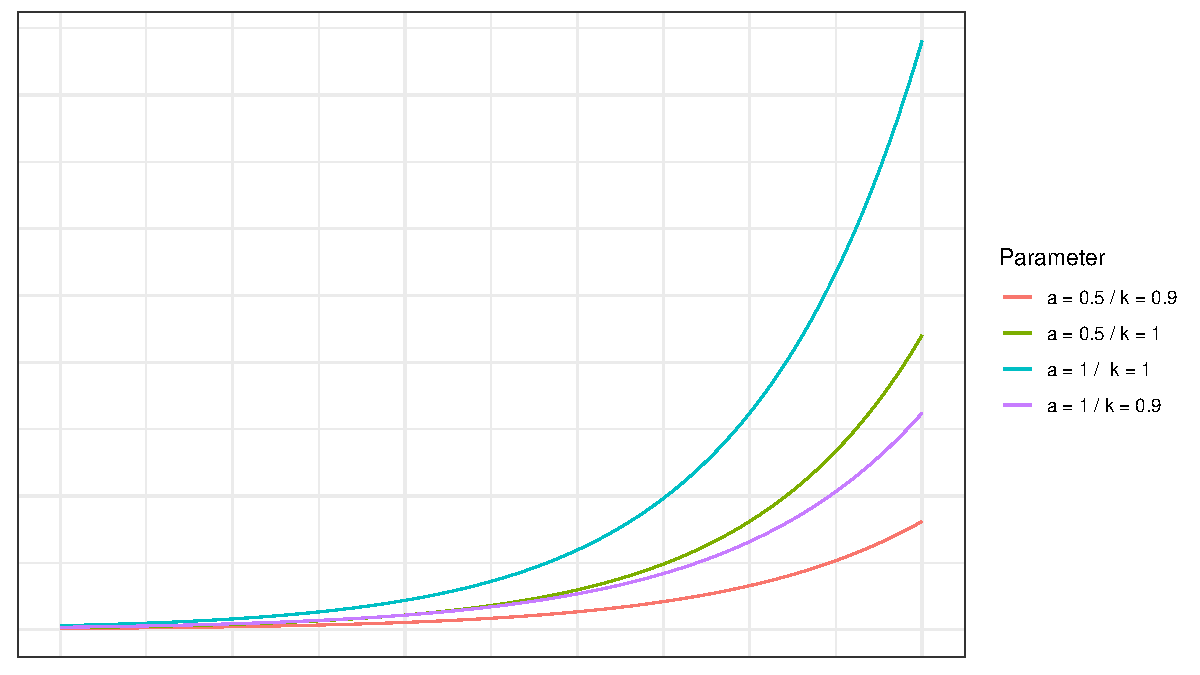
\includegraphics{Learning_R_files/figure-latex/unnamed-chunk-9-1.pdf}
\caption{Exemples de courbes exponetielles selon leurs paramètres}
\end{figure}

On peut aussi imaginer des valeurs négatives de \(k\) pour avoir des
courbes qui tendent vers 0.

\begin{figure}
\centering
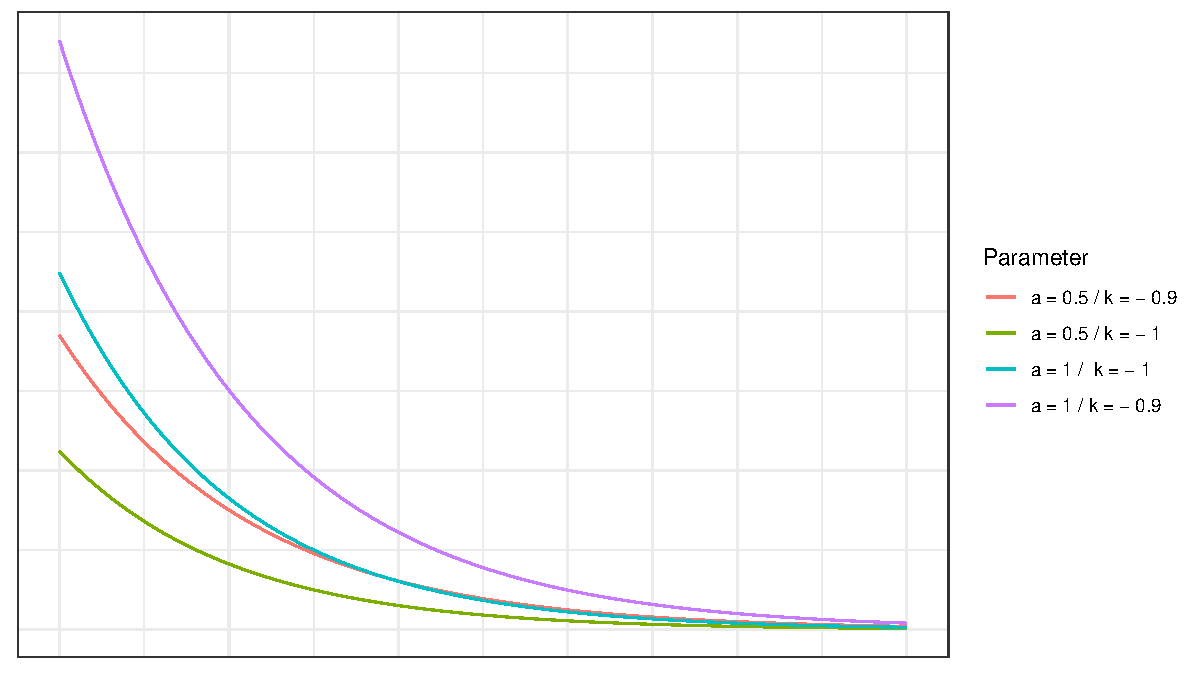
\includegraphics{Learning_R_files/figure-latex/unnamed-chunk-10-1.pdf}
\caption{Exemples de courbes exponetielles avec des coefficients
négatifs}
\end{figure}

\hypertarget{courbe-asymptotique}{%
\paragraph{Courbe asymptotique}\label{courbe-asymptotique}}

On peut représenter des courbes avec un modèle asymptotique pour Y quand
X tend vers l'infini.

\(Y=a-(a-b)e^{-cX}\)

avec :

\begin{itemize}
\tightlist
\item
  \(a\) le maximum possible à atteindre
\item
  \(b\) la valeur de Y à X=0
\item
  \(c\) l'augmentation relative de Y par rapport à X.
\end{itemize}

\begin{figure}
\centering
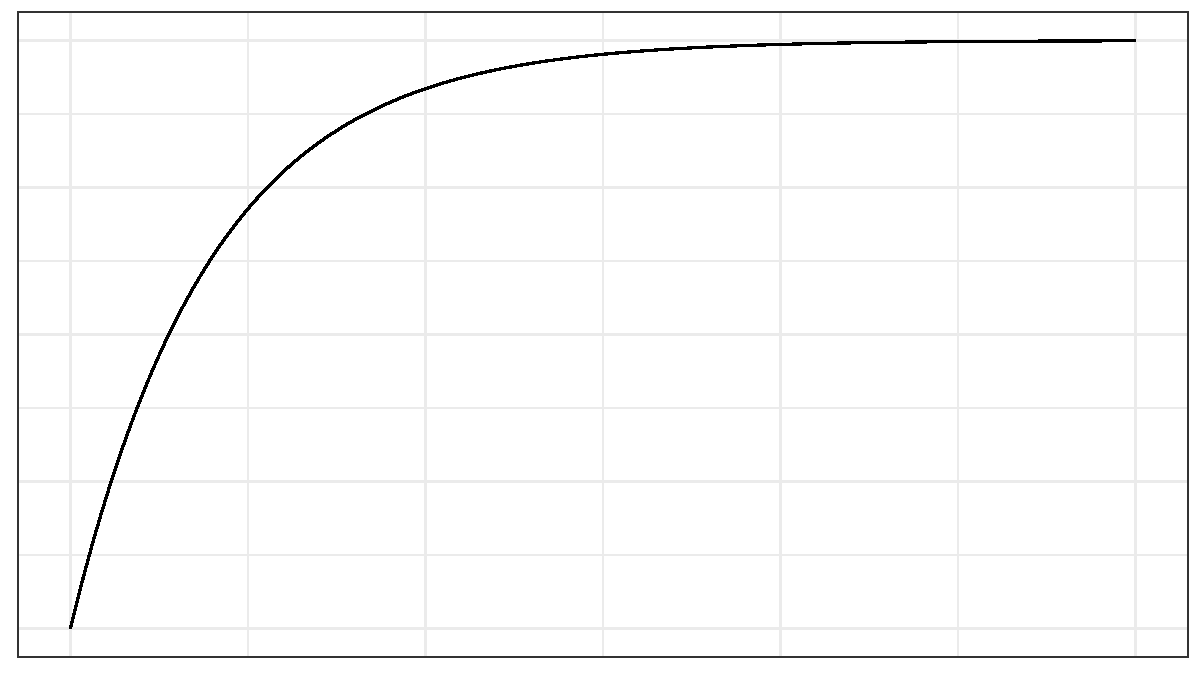
\includegraphics{Learning_R_files/figure-latex/unnamed-chunk-11-1.pdf}
\caption{Exemple de modèle asymptotique}
\end{figure}

Dans le cas particulier où \(b\)=0, on parle souvent d'équation
exponentielle négative, car on obtient alors la formule suivant :

\(Y=a[1-e^{-cX}]\)

On a donc Y=0 quand X=0, on parle alors de \(c\) comme le coefficient
d'extinction.

\hypertarget{courbes-sigmouxefdales}{%
\subsubsection{Courbes sigmoïdales}\label{courbes-sigmouxefdales}}

\(Y=c+\frac{d-c}{1+e^{b(X-e)}}\)

Avec :

\begin{itemize}
\tightlist
\item
  \(d\) : la valeur maximale d'asymptote
\item
  \(c\) : la valeur minimale d'asymptote
\item
  \(e\) : la valeur de X pour laquelle on est à mi-chemin entre \(c\) et
  \(d\)
\item
  \(b\) : représente la pente au niveau du point d'inflexion .
\end{itemize}

\begin{figure}
\centering
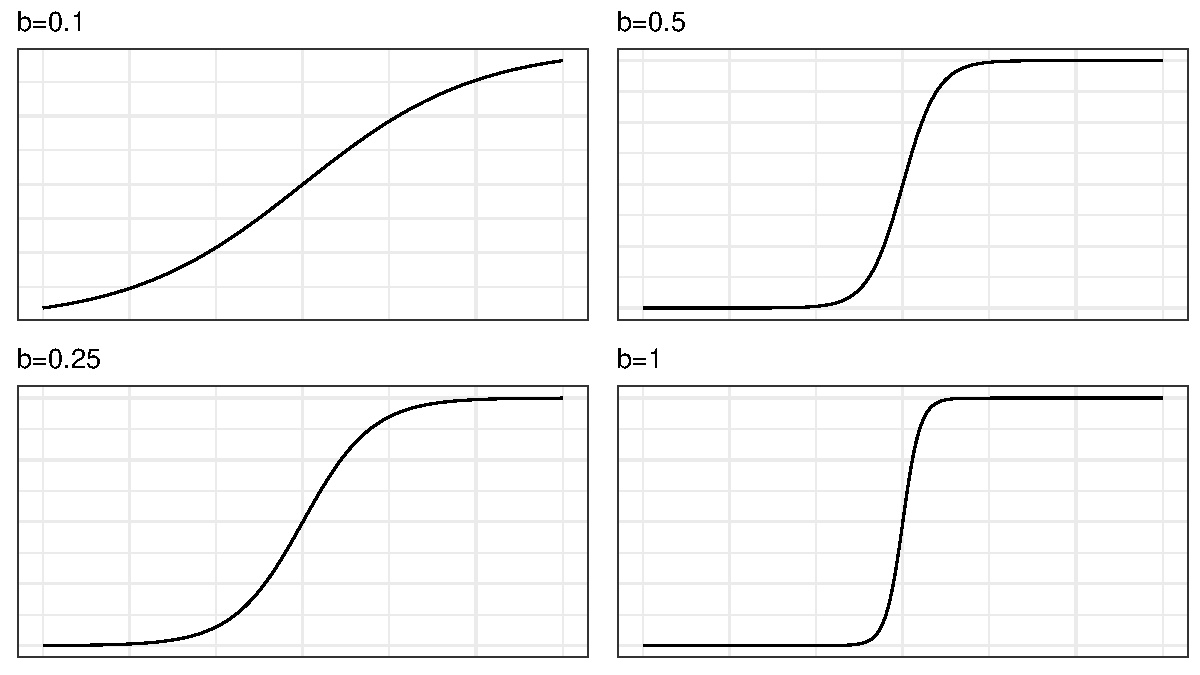
\includegraphics{Learning_R_files/figure-latex/unnamed-chunk-12-1.pdf}
\caption{Exemple du plusieurs courbes de régression logistique pour
différentes valeurs de b}
\end{figure}

Cette fonction est utilisée dans le cadre d'une régression logistique à
quatre paramètres. Dans une cas d'une régression logistique bimodale, on
restreint alors \(c\) à 0 et \(d\) à 1. Il reste alors deux facteurs à
estimer.

\pagebreak

\hypertarget{analyse-factorielle}{%
\section{Analyse Factorielle}\label{analyse-factorielle}}

\hypertarget{analyse-factorielle-1}{%
\section{Analyse Factorielle}\label{analyse-factorielle-1}}

Pour les analyses factorielles, un des packages des plus utilisés est
\emph{FactoMineR}, par sa simplicité, ses graphiques et ses extensions
en clique-bouton en lien avec Rcommander. Pour information, nombreuses
des méthodes implémentées dans ce package ont été codées par leur
créateur (AFM, ACM, etc..). Le package \emph{factoextra} sera aussi
utilisé pour sa complémentarité avec \emph{FactoMineR} et permettant la
réalisation simple de beaux graphiques

catdes() for categories description dimdesc() for dimension description
condes() for Continuous variables descriptions plotellipses() for
confidence ellipses around categories after PCA or MCA

\hypertarget{notion-dinertie}{%
\subsection{Notion d'inertie}\label{notion-dinertie}}

L'inertie d'un jeu de données peut être considérée comme la quantité
d'informations contenue au sein du jeu de données. On définit alors
l'inertie \emph{I} de l'ensemble d'un groupe de données à partir de son
centre de gravité \emph{g} :

\begin{center}
$I=\frac{1}{n}\sum_i^nd(e_i,g)^2$,
\end{center}

avec \emph{d} la distance de chaque individu \(e_i\) au centre de
gravité \emph{g}. Lors de la classification, notamment hiérarchique
ascendante, on peut définir l'inertie intra-classe \(I_a\) (information
contenue dans l'ensemble des groupes) et l'inertie inter-classe \(I_e\)
(information non contenue dans les groupes) à partir des centres de
gravité partiels \(g_i\) de chacun des \emph{k} groupes :

\begin{center}

$I_e=\frac{1}{n}\sum_i^kn_id(g_i,g)^2$

$I_a=\frac{1}{n}\sum_i^k\sum_j^{n_i}d(e_j,g_i)^2$

\end{center}

Si une inertie est nulle, cela signifie que tous les individus sont
identiques. Par définition, l'inertie \(I\) équivaut à la somme des
variances des \emph{j} variables du jeu de données. Si toutes les
données sont centrées-réduites, alors l'inertie vaut \emph{j}

\hypertarget{acp-analyse-en-composante-principale}{%
\subsection{ACP : Analyse en Composante
Principale}\label{acp-analyse-en-composante-principale}}

\hypertarget{cadre}{%
\subsubsection{Cadre}\label{cadre}}

La réalisation d'une ACP permet de répondre à de multiples objectifs :
Permettre une représentation d'un jeu de données complexe en limitant le
nombre de dimensions tout en conservant un maximum d'information, mais
également d'étudier des corrélations multiples de façon simultanée.

Pour présenter l'ACP, on s'aidera du jeu de données \emph{decathlon}
présent dans le package \emph{FactoMineR}. Il représente pour plusieurs
individus leur résultats sur les dix épreuves d'un décathlon, leur
classement à la fin des épreuves, le nombre de points associés et le
cadre dans lequel le décathlon a été réalisé.

\begin{Shaded}
\begin{Highlighting}[]
\FunctionTok{library}\NormalTok{(FactoMineR)}
\FunctionTok{data}\NormalTok{(decathlon)}
\FunctionTok{kable}\NormalTok{(}\FunctionTok{head}\NormalTok{(decathlon[,}\DecValTok{1}\SpecialCharTok{:}\DecValTok{7}\NormalTok{]))}
\end{Highlighting}
\end{Shaded}

\begin{longtable}[]{@{}lrrrrrrr@{}}
\toprule
& 100m & Long.jump & Shot.put & High.jump & 400m & 110m.hurdle &
Discus \\
\midrule
\endhead
SEBRLE & 11.04 & 7.58 & 14.83 & 2.07 & 49.81 & 14.69 & 43.75 \\
CLAY & 10.76 & 7.40 & 14.26 & 1.86 & 49.37 & 14.05 & 50.72 \\
KARPOV & 11.02 & 7.30 & 14.77 & 2.04 & 48.37 & 14.09 & 48.95 \\
BERNARD & 11.02 & 7.23 & 14.25 & 1.92 & 48.93 & 14.99 & 40.87 \\
YURKOV & 11.34 & 7.09 & 15.19 & 2.10 & 50.42 & 15.31 & 46.26 \\
WARNERS & 11.11 & 7.60 & 14.31 & 1.98 & 48.68 & 14.23 & 41.10 \\
\bottomrule
\end{longtable}

Une question qui est posée est si certains sport sont plus discriminants
pour chercher à atteindre les premières places. C'est dans ce cadre
qu'on utilisera l'ACP pour regarder les liens entre variables.

\begin{Shaded}
\begin{Highlighting}[]
\NormalTok{res }\OtherTok{\textless{}{-}} \FunctionTok{PCA}\NormalTok{(decathlon,}\AttributeTok{graph=}\NormalTok{F, }
           \AttributeTok{quanti.sup =} \DecValTok{11}\SpecialCharTok{:}\DecValTok{12}\NormalTok{, }\CommentTok{\# Les variables 11 et 12 sont quantitatives supplémentaires}
           \AttributeTok{quali.sup=}\DecValTok{13}\NormalTok{) }\CommentTok{\# La variable 13  qualitative ne participera pas à la construction des axes.}
\end{Highlighting}
\end{Shaded}

On peut appliquer plusieurs fonctions au résultat obtenu :

\begin{itemize}
\tightlist
\item
  \emph{dimdesc()} fpour la description des dimensions par les variables
\item
  \emph{plotellipses()} pour tracer des ellipses de confiances sur le
  plan factoriel pour les variables qualitatives
\end{itemize}

\hypertarget{ruxe9duire-ou-ne-pas-ruxe9duire-telle-est-la-question}{%
\subsubsection{Réduire ou ne pas réduire, telle est la
question}\label{ruxe9duire-ou-ne-pas-ruxe9duire-telle-est-la-question}}

Avant de lancer l'ACP, une question qui peut se poser est de réduire ou
non les données utilisées. Le centrage est automatique pour permettre de
ramener toutes les variables avec une même moyenne (à savoir 0). La
réduction n'est pas automatique et le fait de la réalisation ou non
influe fortement sur les résultats. La réduction induit que chaque
variable voit sa variance réduite à 1 et donc que toutes les variables
apporteront à l'ACP la même quantité de données. Cela permet notamment
de comparer des variables quantitatives non comparables en temps normal,
comme c'est le cas ici. Comparer un temps aux 100 mètres en seconde et
une longueur de saut en mètre n'a pas vraiment de sens et donc la
question ne se pose pas. Cependant, si les variables sont dans la même
unité, la question revient à savoir si on souhaite permettre que chaque
variable apporte la même quantité d'information ou si on souhaite que
celles avec de plus grandes variances soient de bases discriminantes. .

\hypertarget{ac-analyse-des-correspondances}{%
\subsection{AC : Analyse des
Correspondances}\label{ac-analyse-des-correspondances}}

\hypertarget{acm-analyse-des-correspondances-multiples}{%
\subsection{ACM : Analyse des Correspondances
Multiples}\label{acm-analyse-des-correspondances-multiples}}

équivalent l'ACP pour données que qualitatives

\hypertarget{afdm-analyse-factorielle-de-donnuxe9es-mixtes}{%
\subsection{AFDM : Analyse Factorielle de Données
Mixtes}\label{afdm-analyse-factorielle-de-donnuxe9es-mixtes}}

méthode permettent d'utiliser des données quali et quanti dans un même
tableau d'analyse

\hypertarget{afm-analyse-factorielle-multiple}{%
\subsection{AFM: Analyse Factorielle
Multiple}\label{afm-analyse-factorielle-multiple}}

\begin{Shaded}
\begin{Highlighting}[]
\FunctionTok{data}\NormalTok{(wine)}
\NormalTok{res }\OtherTok{\textless{}{-}} \FunctionTok{MFA}\NormalTok{(wine, }\AttributeTok{group=}\FunctionTok{c}\NormalTok{(}\DecValTok{2}\NormalTok{,}\DecValTok{5}\NormalTok{,}\DecValTok{3}\NormalTok{,}\DecValTok{10}\NormalTok{,}\DecValTok{9}\NormalTok{,}\DecValTok{2}\NormalTok{), }\AttributeTok{type=}\FunctionTok{c}\NormalTok{(}\StringTok{"n"}\NormalTok{,}\FunctionTok{rep}\NormalTok{(}\StringTok{"s"}\NormalTok{,}\DecValTok{5}\NormalTok{)),}
    \AttributeTok{ncp=}\DecValTok{5}\NormalTok{, }\AttributeTok{name.group=}\FunctionTok{c}\NormalTok{(}\StringTok{"orig"}\NormalTok{,}\StringTok{"olf"}\NormalTok{,}\StringTok{"vis"}\NormalTok{,}\StringTok{"olfag"}\NormalTok{,}\StringTok{"gust"}\NormalTok{,}\StringTok{"ens"}\NormalTok{),}
    \AttributeTok{num.group.sup=}\FunctionTok{c}\NormalTok{(}\DecValTok{1}\NormalTok{,}\DecValTok{6}\NormalTok{),}\AttributeTok{graph=}\NormalTok{F)}
\end{Highlighting}
\end{Shaded}

Dual MFA et AFMH en supplément

\hypertarget{gpa}{%
\subsection{GPA :}\label{gpa}}

\hypertarget{analyse-canonique}{%
\subsection{Analyse Canonique}\label{analyse-canonique}}

\pagebreak

\hypertarget{ruxe9gression}{%
\section{Régression}\label{ruxe9gression}}

Documents sources utilisés:

\begin{itemize}
\item
  \href{http://r-statistics.co/Linear-Regression.html}{\textcolor{blue}{Linear Regression}},
  via le site R-statistics.co
\item
  \href{https://pbil.univ-lyon1.fr/R/pdf/br4.pdf}{\textcolor{blue}{Modèle Linéaire}},
  D. Chessel \& J. Thioulouse, Université de Lyon 1
\item
  Plusieurs cours d'Agrocampus Ouest (document Perso)
\end{itemize}

\hypertarget{moduxe8le-linuxe9aire-ruxe9gression-simple-multiple-anova-et-ancova}{%
\subsection{Modèle Linéaire : Régression simple, multiple, Anova et
Ancova}\label{moduxe8le-linuxe9aire-ruxe9gression-simple-multiple-anova-et-ancova}}

Le modèle linéaire classique (LM for linear model) est celui le plus
utilisé. Il permet de lier une variable réponse à une ou plusieurs
variables explicatives. On a tendance à découper beaucoup de modèle
dedans, Anova, régression simple, régression multiple ou ANVOCA. Au
final, toutes ces approches sont toutes issues d'une même théorie, le
modèle linéare. Dans ce cas, la variable réponse est quantitative, c'est
cela qui regroupe ces modèles, et suit une loi Normale. Du coup, quelles
différences entre ces éléments ?

\begin{itemize}
\tightlist
\item
  ANOVA : Analyse de l'effet d'un ou plusieurs facteurs qualitatif
\item
  Régression simple : Analyse de l'effet d'une variable quantitative
\item
  Régression multiple : Analyse de l'effet de plusieurs variables
  quantitatives
\item
  ANCOVA : Analyse de l'effet de plusieurs facteurs , avec des variables
  qualitatives et quantitatives
\end{itemize}

Un petit exemple, on cherche à la distance de freinage à la vitesse d'un
véhicule (jeu de données cars)

\begin{Shaded}
\begin{Highlighting}[]
\FunctionTok{library}\NormalTok{(ggplot2) }\CommentTok{\# pour les graphiques}
\FunctionTok{data}\NormalTok{(cars) }
\FunctionTok{str}\NormalTok{(cars) }\CommentTok{\# Avoir un apercu des données, et notamment de leur natures}
\end{Highlighting}
\end{Shaded}

\begin{verbatim}
% 'data.frame': 50 obs. of  2 variables:
%  $ speed: num  4 4 7 7 8 9 10 10 10 11 ...
%  $ dist : num  2 10 4 22 16 10 18 26 34 17 ...
\end{verbatim}

\begin{Shaded}
\begin{Highlighting}[]
\NormalTok{mod}\OtherTok{\textless{}{-}}\FunctionTok{lm}\NormalTok{(dist}\SpecialCharTok{\textasciitilde{}}\NormalTok{speed,}\AttributeTok{data=}\NormalTok{cars) }\CommentTok{\# Modèle linéaire}
\NormalTok{p}\OtherTok{\textless{}{-}}\FunctionTok{ggplot}\NormalTok{(}\AttributeTok{data=}\NormalTok{cars,}\FunctionTok{aes}\NormalTok{(}\AttributeTok{x=}\NormalTok{speed,}\AttributeTok{y=}\NormalTok{dist))}\SpecialCharTok{+}\FunctionTok{geom\_point}\NormalTok{()}\SpecialCharTok{+}
  \FunctionTok{theme\_classic}\NormalTok{()}\SpecialCharTok{+}\FunctionTok{labs}\NormalTok{(}\AttributeTok{x=}\StringTok{"Vitesse du véhicule"}\NormalTok{,}\AttributeTok{y=}\StringTok{"Distance de freinage"}\NormalTok{)}\SpecialCharTok{+}
  \FunctionTok{geom\_smooth}\NormalTok{(}\AttributeTok{method=}\StringTok{"lm"}\NormalTok{) }\CommentTok{\# Permet d\textquotesingle{}avoir une estimation de la pente de régression linéaire}
\FunctionTok{print}\NormalTok{(p)}
\end{Highlighting}
\end{Shaded}

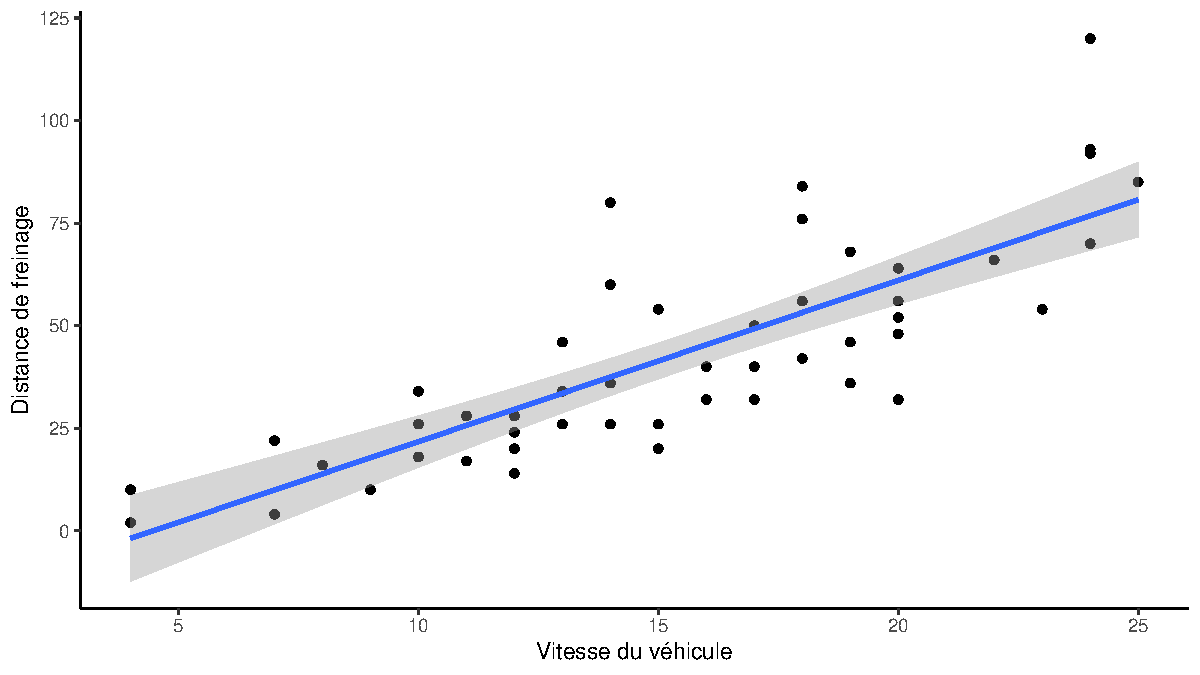
\includegraphics{Learning_R_files/figure-latex/unnamed-chunk-30-1.pdf}

\hypertarget{un-choix-anodin-mais-primordial-les-contrastes}{%
\subsubsection{Un choix anodin mais primordial : les
contrastes}\label{un-choix-anodin-mais-primordial-les-contrastes}}

Un élément très important lors de toutes les régressions est le choix
des contrastes. Il existe plusieurs façons d'aborder les contrastes lors
des modèles, particulièrement d'Anova :

\begin{itemize}
\tightlist
\item
  contr.sum se traduit en statistique par \(\sum_i\alpha_i=0\)
  (Statistiques à la française)
\item
  contr.treatment se traduit en statistique par \(alpha_1=0\). Dans ce
  cas, l'estimation de la moyenne (l'intercept) se fait donc pour le
  niveau 1 de toutes les valeurs observées en ANOVA. (Statistiques à
  l'anglo-saxonne)
\item
  contr.helmert : returns Helmert contrasts, which contrast the second
  level with the first, the third with the average of the first two, and
  so on
\end{itemize}

C'est important si on veut intérpréter les coefficients directement, à
partir des sorties du modèle linéaire, notamment sur des variables
qualitatives. MAis on peut passer cette étape à l'aide de package.

\begin{Shaded}
\begin{Highlighting}[]
\FunctionTok{summary}\NormalTok{(mod)}
\end{Highlighting}
\end{Shaded}

\begin{verbatim}
% 
% Call:
% lm(formula = dist ~ speed, data = cars)
% 
% Residuals:
%     Min      1Q  Median      3Q     Max 
% -29.069  -9.525  -2.272   9.215  43.201 
% 
% Coefficients:
%             Estimate Std. Error t value Pr(>|t|)    
% (Intercept) -17.5791     6.7584  -2.601   0.0123 *  
% speed         3.9324     0.4155   9.464 1.49e-12 ***
% ---
% Signif. codes:  0 '***' 0.001 '**' 0.01 '*' 0.05 '.' 0.1 ' ' 1
% 
% Residual standard error: 15.38 on 48 degrees of freedom
% Multiple R-squared:  0.6511,  Adjusted R-squared:  0.6438 
% F-statistic: 89.57 on 1 and 48 DF,  p-value: 1.49e-12
\end{verbatim}

Cette sortie donne la moyenne pour une vitesse nulle est de -17.58, et
on prend 3.93 m de freinage tous les 1km/h gagnés.

\hypertarget{estimation-des-coefficients}{%
\subsection{Estimation des
coefficients}\label{estimation-des-coefficients}}

On va profiter du jeu de données \emph{diamonds} pour cela. On va
s'intéresser à l'effet du poids, de la taill, la couleur et de sa
clareté sur le prix

\begin{Shaded}
\begin{Highlighting}[]
\FunctionTok{data}\NormalTok{(}\StringTok{"diamonds"}\NormalTok{)}
\NormalTok{mod}\OtherTok{=}\FunctionTok{lm}\NormalTok{(price}\SpecialCharTok{\textasciitilde{}}\NormalTok{cut}\SpecialCharTok{+}\NormalTok{color}\SpecialCharTok{+}\NormalTok{clarity}\SpecialCharTok{+}\NormalTok{carat,diamonds)}
\FunctionTok{library}\NormalTok{(car)}
\FunctionTok{Anova}\NormalTok{(mod,}\AttributeTok{type=}\StringTok{"III"}\NormalTok{)}
\end{Highlighting}
\end{Shaded}

\begin{verbatim}
% Anova Table (Type III tests)
% 
% Response: price
%                 Sum Sq    Df   F value    Pr(>F)    
% (Intercept) 9.4276e+10     1  70444.50 < 2.2e-16 ***
% cut         1.6992e+09     4    317.41 < 2.2e-16 ***
% color       1.6320e+10     6   2032.46 < 2.2e-16 ***
% clarity     3.8452e+10     7   4104.51 < 2.2e-16 ***
% carat       7.2976e+11     1 545289.36 < 2.2e-16 ***
% Residuals   7.2163e+10 53921                        
% ---
% Signif. codes:  0 '***' 0.001 '**' 0.01 '*' 0.05 '.' 0.1 ' ' 1
\end{verbatim}

On peut voir que toutes les variables sont ultra signigicatifes, avec
des probabilités en deça de la limiete de calcul de R (2.2e-16).

Comment avoir des estimer des moyennes pour chaque niveau de facteur

\begin{Shaded}
\begin{Highlighting}[]
\FunctionTok{library}\NormalTok{(emmeans)}
\FunctionTok{emmeans}\NormalTok{(mod,}\StringTok{"cut"}\NormalTok{)}
\end{Highlighting}
\end{Shaded}

\begin{verbatim}
%  cut       emmean   SE    df lower.CL upper.CL
%  Fair        2706 29.4 53921     2648     2763
%  Good        3361 17.8 53921     3326     3396
%  Very Good   3554 12.5 53921     3530     3579
%  Premium     3575 12.0 53921     3551     3599
%  Ideal       3704 10.1 53921     3684     3724
% 
% Results are averaged over the levels of: color, clarity 
% Confidence level used: 0.95
\end{verbatim}

et si on croise

\begin{Shaded}
\begin{Highlighting}[]
\NormalTok{mod2}\OtherTok{=}\FunctionTok{lm}\NormalTok{(price}\SpecialCharTok{\textasciitilde{}}\NormalTok{(cut}\SpecialCharTok{+}\NormalTok{color}\SpecialCharTok{+}\NormalTok{clarity)}\SpecialCharTok{\^{}}\DecValTok{2}\SpecialCharTok{+}\NormalTok{carat,diamonds) }
\CommentTok{\# le \^{}2 permet de tester toutes les combinaisons de niveau 2 au max}

\FunctionTok{emmeans}\NormalTok{(mod2,}\FunctionTok{c}\NormalTok{(}\StringTok{"cut"}\NormalTok{,}\StringTok{"color"}\NormalTok{))}
\end{Highlighting}
\end{Shaded}

\begin{verbatim}
%  cut       color emmean    SE    df lower.CL upper.CL
%  Fair      D       3935 108.0 53827     3724     4146
%  Good      D       4629  57.2 53827     4517     4742
%  Very Good D       4807  43.5 53827     4722     4893
%  Premium   D       4975  42.5 53827     4892     5059
%  Ideal     D       4962  36.5 53827     4890     5033
%  Fair      E       3611  99.0 53827     3416     3805
%  Good      E       4158  46.4 53827     4067     4249
%  Very Good E       4285  32.1 53827     4222     4348
%  Premium   E       4418  32.1 53827     4355     4481
%  Ideal     E       4351  27.8 53827     4297     4406
%  Fair      F       3486  85.6 53827     3318     3654
%  Good      F       3892  45.6 53827     3803     3981
%  Very Good F       4183  32.3 53827     4120     4247
%  Premium   F       4231  30.6 53827     4171     4291
%  Ideal     F       4313  23.7 53827     4267     4360
%  Fair      G       2896  86.7 53827     2726     3066
%  Good      G       3591  45.0 53827     3503     3679
%  Very Good G       3842  31.1 53827     3781     3903
%  Premium   G       3913  26.6 53827     3861     3965
%  Ideal     G       4054  23.5 53827     4008     4100
%  Fair      H       2201  90.8 53827     2023     2379
%  Good      H       3257  51.0 53827     3157     3357
%  Very Good H       3319  34.9 53827     3251     3387
%  Premium   H       3254  29.9 53827     3195     3312
%  Ideal     H       3531  25.3 53827     3482     3581
%  Fair      I       1884 107.0 53827     1675     2093
%  Good      I       2677  58.1 53827     2563     2791
%  Very Good I       2897  42.1 53827     2815     2980
%  Premium   I       2834  37.5 53827     2760     2907
%  Ideal     I       3116  32.2 53827     3053     3180
%  Fair      J       1055 125.0 53827      809     1300
%  Good      J       1869  76.5 53827     1719     2019
%  Very Good J       2085  56.5 53827     1974     2195
%  Premium   J       1868  52.2 53827     1766     1970
%  Ideal     J       2287  51.0 53827     2187     2387
% 
% Results are averaged over the levels of: clarity 
% Confidence level used: 0.95
\end{verbatim}

Et si on veut savoir les niveaux qui se recoupent ?

\begin{Shaded}
\begin{Highlighting}[]
\FunctionTok{library}\NormalTok{(multcomp)}
\FunctionTok{cld}\NormalTok{(}\FunctionTok{emmeans}\NormalTok{(mod2,}\FunctionTok{c}\NormalTok{(}\StringTok{"cut"}\NormalTok{)))}
\end{Highlighting}
\end{Shaded}

\begin{verbatim}
%  cut       emmean   SE    df lower.CL upper.CL .group
%  Fair        2724 65.8 53827     2595     2853  1    
%  Good        3439 28.9 53827     3382     3496   2   
%  Very Good   3631 21.0 53827     3590     3673    3  
%  Premium     3642 17.7 53827     3607     3676    3  
%  Ideal       3802 15.8 53827     3771     3833     4 
% 
% Results are averaged over the levels of: color, clarity 
% Confidence level used: 0.95 
% P value adjustment: tukey method for comparing a family of 5 estimates 
% significance level used: alpha = 0.05 
% NOTE: If two or more means share the same grouping symbol,
%       then we cannot show them to be different.
%       But we also did not show them to be the same.
\end{verbatim}

\hypertarget{lanalyse-de-variance}{%
\subsection{L'analyse de Variance}\label{lanalyse-de-variance}}

\hypertarget{moduxe8les-uxe0-effet-fixe}{%
\subsection{Modèles à effet fixe}\label{moduxe8les-uxe0-effet-fixe}}

L'objectif est d'expliquer une variable quantitative par des variables
qualitatives, aussi appelées facteurs (à plusieurs modalités). Cela
revient donc à expliquer la variabilité . Celle-ci se mesure par sa
dispersion, et se quantifie par sa variance.

\hypertarget{analyse-de-variance-uxe0-un-facteur}{%
\subsubsection{Analyse de variance à un
facteur}\label{analyse-de-variance-uxe0-un-facteur}}

\hypertarget{moduxe8le-mixte}{%
\subsubsection{Modèle Mixte}\label{moduxe8le-mixte}}

Explication des effets aléatoires

\begin{Shaded}
\begin{Highlighting}[]
\FunctionTok{library}\NormalTok{(lme4)}
\FunctionTok{library}\NormalTok{(emmeans)}
\FunctionTok{data}\NormalTok{(}\StringTok{"Theoph"}\NormalTok{)}
\NormalTok{mod}\OtherTok{\textless{}{-}}\FunctionTok{lmer}\NormalTok{(conc}\SpecialCharTok{\textasciitilde{}}\NormalTok{Subject}\SpecialCharTok{+}\NormalTok{(}\DecValTok{1}\SpecialCharTok{|}\NormalTok{Time),}\AttributeTok{data=}\NormalTok{Theoph)}
\CommentTok{\# mod$residuals}
\FunctionTok{resid}\NormalTok{(mod)}
\end{Highlighting}
\end{Shaded}

\begin{verbatim}
%            1            2            3            4            5            6 
% -1.058248092 -1.500667320 -0.065553428  1.004809869  0.486435289  0.481884289 
%            7            8            9           10           11           12 
%  0.421965733  0.603905533  0.021600835  0.565475490 -0.961608198 -0.080718408 
%           13           14           15           16           17           18 
% -1.217214356  2.468593253 -0.117960850  0.881576378 -0.322332706  0.072475212 
%           19           20           21           22           23           24 
%  0.251435217 -0.197441006 -0.596376060 -1.142036675 -0.688350630  0.855153422 
%           25           26           27           28           29           30 
%  1.035643117  1.448867553 -0.263667248  0.490027074  0.135962879 -0.746957090 
%           31           32           33           34           35           36 
% -0.455073227 -0.544929803 -1.266676047 -0.191733244 -0.902638848 -0.164551180 
%           37           38           39           40           41           42 
%  0.924877112  0.864958556  0.256652459  0.761460377 -0.202894055  0.034269483 
%           43           44           45           46           47           48 
% -0.276217580 -1.104183082 -0.804470031 -3.131706720 -0.535158370  2.248287527 
%           49           50           51           52           53           54 
%  1.150213350  0.843915672  0.828723590  0.494369158  0.022629817  0.039872317 
%           55           56           57           58           59           60 
% -1.156676309  1.121585614 -0.444910334 -0.974420640  0.694277515  0.661594666 
%           61           62           63           64           65           66 
%  0.446432578 -0.423515637  0.035173398 -0.117346563 -0.189737067 -0.809133529 
%           67           68           69           70           71           72 
%  0.949834207 -0.892585020 -1.489459361 -0.242947609  0.004517589  0.783678341 
%           73           74           75           76           77           78 
%  0.974732957  0.282541326  0.523111610 -0.059301365 -0.834122673  0.507602521 
%           79           80           81           82           83           84 
%  1.015183293 -1.803085818  0.456695298  0.692285902  0.993186130 -0.470740263 
%           85           86           87           88           89           90 
%  0.061324281  0.017747150 -0.583720161 -0.886478333 -0.140042932  2.882720379 
%           91           92           93           94           95           96 
%  1.056068876  0.541314008 -1.185359551 -0.584459323 -0.396849312 -0.248521504 
%           97           98           99          100          101          102 
% -0.283927924 -0.542667143 -1.098275572 -0.919995160 -0.893994756 -0.259402776 
%          103          104          105          106          107          108 
% -0.812776977  0.451449185  1.099659019  1.161662056  0.503197028  0.263522804 
%          109          110          111          112          113          114 
%  0.428682159 -1.022002581 -0.216756188  2.100824584  2.383950243  0.422336589 
%          115          116          117          118          119          120 
%  0.430542776  0.174527127 -0.923562567 -0.834602563 -1.244245586 -1.103032606 
%          121          122          123          124          125          126 
% -1.189981809 -0.354866635 -1.647285862 -1.034160203 -0.882109076  1.185486501 
%          127          128          129          130          131          132 
%  1.193657214  0.872275867  0.876526906  1.107643968 -0.174002206 -1.143166473
\end{verbatim}

\begin{Shaded}
\begin{Highlighting}[]
\FunctionTok{emmeans}\NormalTok{(mod,}\FunctionTok{c}\NormalTok{(}\StringTok{"Subject"}\NormalTok{))}
\end{Highlighting}
\end{Shaded}

\begin{verbatim}
%  Subject emmean    SE    df lower.CL upper.CL
%  6         3.89 0.637 110.3     2.63     5.15
%  7         4.21 0.579  95.6     3.06     5.36
%  8         4.50 0.581  95.5     3.35     5.66
%  11        5.23 0.588  97.5     4.06     6.40
%  3         5.70 0.597  99.6     4.52     6.88
%  2         5.09 0.572  93.1     3.96     6.23
%  4         5.20 0.650 114.4     3.92     6.49
%  9         5.15 0.625 108.2     3.91     6.39
%  12        5.37 0.606 101.8     4.17     6.57
%  10        6.17 0.651 114.4     4.88     7.46
%  1         6.81 0.621 107.4     5.58     8.04
%  5         5.82 0.579  95.2     4.67     6.97
% 
% Degrees-of-freedom method: kenward-roger 
% Confidence level used: 0.95
\end{verbatim}

\hypertarget{moduxe8le-hiuxe9rarchique}{%
\subsubsection{Modèle Hiérarchique}\label{moduxe8le-hiuxe9rarchique}}

l'aléatoire c'est pas assez complexe

\hypertarget{moduxe8le-linuxe9aire-guxe9nuxe9ralisuxe9}{%
\subsection{Modèle Linéaire
Généralisé}\label{moduxe8le-linuxe9aire-guxe9nuxe9ralisuxe9}}

\hypertarget{ruxe9gression-curvilinuxe9aire}{%
\subsection{Régression
Curvilinéaire}\label{ruxe9gression-curvilinuxe9aire}}

\hypertarget{ruxe9gression-non-linuxe9aire}{%
\subsection{Régression
non-linéaire}\label{ruxe9gression-non-linuxe9aire}}

\hypertarget{exemples-dapplications}{%
\subsubsection{Exemples d'applications}\label{exemples-dapplications}}

\hypertarget{moduxe8le-systuxe8mique}{%
\paragraph{Modèle systèmique}\label{moduxe8le-systuxe8mique}}

On s'intéresse à la dynamique de la digestion d'une molécule chez un
poisson. Pour cela, on suit la position de la molécule dans les
différentes parties des poissons. On obtient un modèle à 3
compartiments, où la molécule peut avancer selon le schéma présenté
après. On obtient alors à 3 équations différnetielle, pour expliquer la
dynamique de transfert entre compartiments, comme représenté sur la
figure \ref{CinBio}.

\begin{figure}
  \centering
  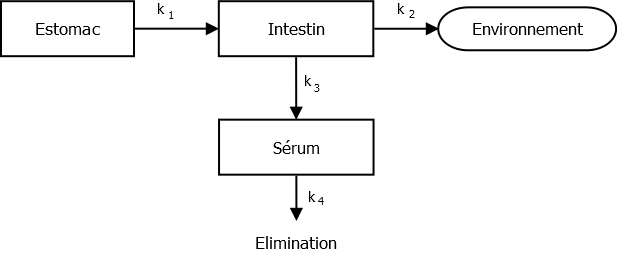
\includegraphics{Regression/Model_Cin_Bio.png}
  \caption{Modèle cinétique biologique}
  \label{CinBio}
\end{figure}

On obtient alors trois équations différentielles pour exprimer
l'évolution de la molécule dans les compartiments qui nous intéressent :

\begin{itemize}
\tightlist
\item
  Estomac : \(\frac{dq_1}{dt}=-k_1q_1(t)\)
\item
  Intestin : \(\frac{dq_2}{dt} =k_1q_1(t)-[k_2+k_3]q_2(t)\)
\item
  Sérum : \(\frac{dq_3}{dt}=k_3q_2(t)-k_4q_3(t)\)
\end{itemize}

Si on les résoud, on obtient alors :

\begin{itemize}
\tightlist
\item
  Estomac : \(q_1(t)=q_0e^{-k_1t}\)
\item
  Intestin : \(q_2(t)=\frac{k_1q_0}{k_2+k_3-k_1}f_1(t)\)
\item
  Sérum :\(q_3(t)=f_3(t)\)
\end{itemize}

où \(f_1(t)\) et \(f_2(t)\) sont des fonctions non-linéaires du temps.
On ne peut donc pas réaliser une régression linéaire pour estimer ces
deux fonctions. On obtient donc le problème que les systèmes
non-linéaires, les méthodes vues précédemment ne sont donc pas
applicables. Il faut chercher un autre moyen d'expliquer la variable
réponse à partir des variables explicatives.

\hypertarget{moduxe9lisation-allomuxe9trique}{%
\paragraph{Modélisation
allométrique}\label{moduxe9lisation-allomuxe9trique}}

La modélisation allométrique est souvent utilisée pour suivre
l'évolution de la part d'un animal (organe, muscles, lipides, etc..) par
rapport au poids/volume total. Par exemple, on suit ici l'évolution du
poids des lipides par rapport au poids d'un animal. On obtient souvent
des équations de la forme :

\begin{center}
$\frac{d( \frac{Y}{x})}{dx}= \beta_{1} \frac{Y}{x}$
\end{center}

ce qui donne après résolution :
\(Y= \beta_{0}x_{1}^{\beta_{}}+ \epsilon_{i}\). Selon la valeur de beta,
plusieurs types de croissances sont distinguables (tardive, isométrique
ou précose, dans l'ordre croissant)

\hypertarget{cinuxe9tique-en-biochimie}{%
\paragraph{Cinétique en biochimie}\label{cinuxe9tique-en-biochimie}}

Quand on étudie de la cinétique, en biochimie notamment, on étudie
également des des modèles non-linéaires. (Il ne faut pas cependant la
non-linéarité quand on sait faire en linéaire). Pax exemple, on
s'intéresse à la décompostion du \(\beta\)-lactose selon différentes
concentrations en NaCl

\begin{figure}
\centering
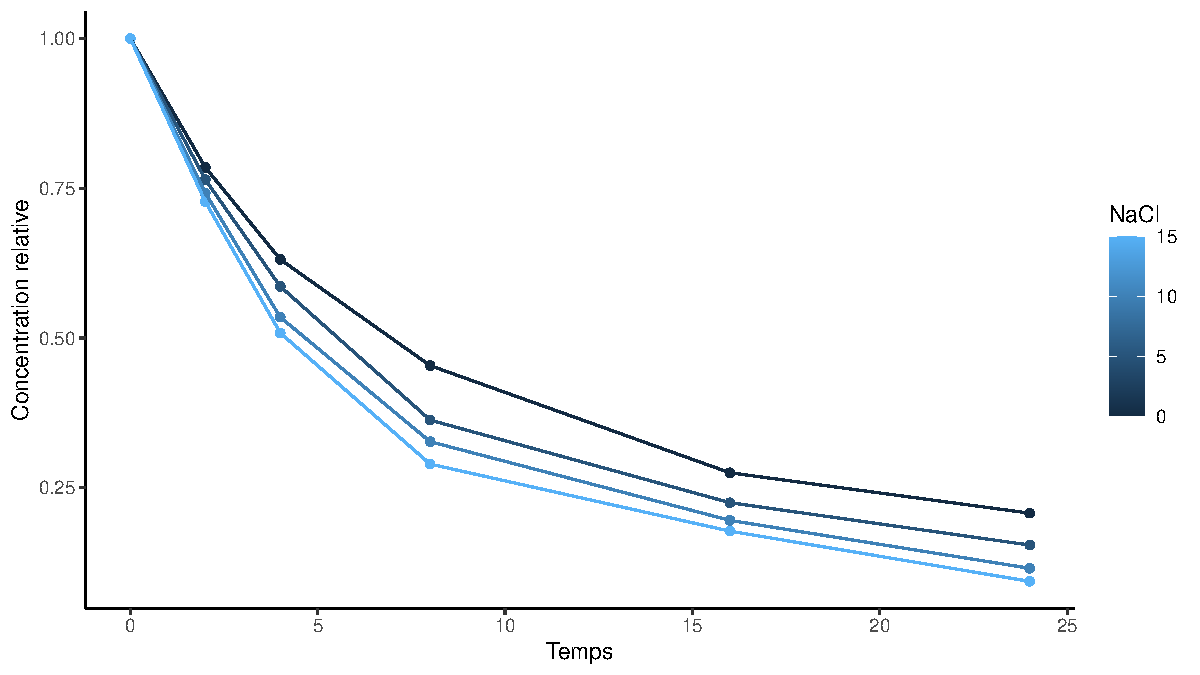
\includegraphics{Learning_R_files/figure-latex/unnamed-chunk-37-1.pdf}
\caption{Evolution de la concentration relative en fonction du temps}
\end{figure}

On s'intéresse à l'évolution de la concentration en lactose en fonction
du temps, en évolution relative. Pour cela, on utilise le modèle suivant
, avec \(Y_{t}\) la concentration en \(\beta\)-lactose à l'instant
\(t\).

\begin{center}
$\frac{dY_{t}}{dt}=-kY_{t}^{\mu}$

$Y_{t}=Y_{0}[1+( \mu-1)kY_{0}^{\mu-1}t]^{\frac{1}{1- \mu}}+ \epsilon_{t}$

$\epsilon \hookrightarrow N(0; \sigma)$
\end{center}

où \(\mu\) et \(k\) dépendent des conditions expérimentales.
\(1 \le \mu \le 2\), k\textgreater0.

On a 2 paramètres inconnues : \(k\) et \(\mu\), 1 seule variable
explicative \(t\).

\begin{center}
$Y_{t}=f(t,k, \mu)+ \epsilon_{t}$
\end{center}

Il faut transformer cela, ici on teste avec le log.

\begin{center}
$log(Y_{t})=log(Y_{0})+log([1+( \mu-1)kY_{0}^{\mu-1}t]^{\frac{1}{1- \mu}}+ \epsilon_{t})$
\end{center}

Mais cela ne marche pas. Il faut chercher la valeur qui minimise l'écart
au modèle

\begin{center}
$SC(k, \mu)= \sum_{i=1}^{n}(Y_{t_{i}}-f(t_{i},k, \mu))^2$
\end{center}

\hypertarget{base-de-la-ruxe9gression}{%
\subsubsection{Base de la régression}\label{base-de-la-ruxe9gression}}

\hypertarget{moduxe8le}{%
\paragraph{Modèle}\label{moduxe8le}}

\begin{center}
$Y=f(x^{1},x^{2},...,x^{p}; \beta_{1}, \beta_{2},..., \beta_{q})+ \epsilon$, où $\epsilon \hookrightarrow N(0, \sigma)$

$Y= \hookrightarrow N[f(x^{1},x^{2},...,x^{p}, \sigma]$
\end{center}

Où la fonction \(f\) est ma surface de réponse du modèle.

Dans le cas du modèle allométrique, on obtient la formule suivante :
\(Y= \beta_{0}x_{1}^{\beta_{}}+ \epsilon_{i}\)

Mais attention, cela est différent de
\(log(Y)=log( \beta_{0})+ \beta_{1}log(x)+ \epsilon\)

\hypertarget{estimation-des-paramuxe8tres}{%
\paragraph{Estimation des
paramètres}\label{estimation-des-paramuxe8tres}}

Pour estimer les paramètres, on utilise le critère des moindres carrés.

\begin{center}
$SC( \beta)= \sum_{i=1}^{n}[Y_{i}-f(x_{i}; \beta)]^2$
\end{center}

On obtient que la dérivée partielle de la somme des carrés par rapport à
chaque coefficient \(\beta\) est nulle. Par exemple, dans le cas
allométrique, on obtient les deux équations estimantes :

\begin{center}
 $-2 \sum_{i=1}^{n}x_{i}^{ \hat{ \beta}_{1}}[Y_{i}- \hat{ \beta}_{0}x_{i}^{ \hat{ \beta}_{1}}]=0$

$-2 \sum_{i=1}^{n} \hat{ \beta}_{0}x_{i}^{ \hat{ \beta}_{1}}log(x_{i})[Y_{i}- \hat{ \beta}_{0}x_{i}^{ \hat{\beta}_{1}}]=0$
\end{center}

Initialisation de l'algorithme d'estimation

On prend l'exemple de NaCl :

Pour trouver le résultat, il faut passer aux dérivées partielles (par
rapport à \(k\) et \(\mu\)). Cependant, quand on cherche à résoudre les
équations à 2 inconnues, il n'y a pas de solution évidente. On va
chercher la fonction à l'aide d'un algorithme pour optimiser ce critère.
Le problème est de trouver \(k\) et \(\mu\) qui annulent la fonction. Il
'agit de l'algorithme de Newton-Raphson. Pour cela, on utilise les
tangeantes et leur propriété mathématiques. On calcule la pente de la
tangeante à un point, on prend le point d'intersection avec les
abcisses, on calcule alors la pente de la tangeante au point associée à
cette valeur de x. On continue jusqu'à ce que le point obtenu soit celui
de l'intersection avec les abcisses pour la fonction. On utilise le
non-linear least squares, nls dans R.On va travailer sur la
concentration relative plutot que sur la concentration réele.

\begin{figure}
  \centering
  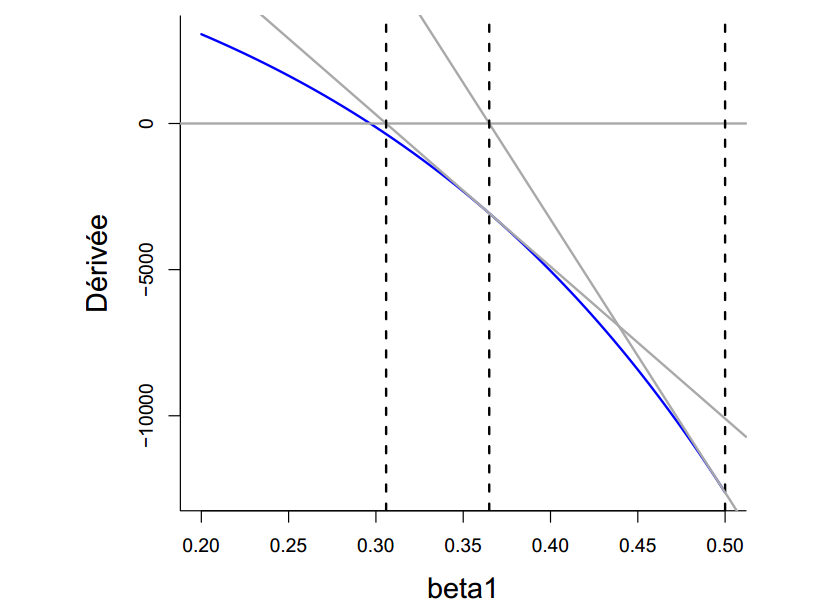
\includegraphics{Regression/Newton-Raphson.png}
  \caption{Schema de résolution par l'algorithme de Newton-raphson}
  \label{NewtonRaphson}
\end{figure}

Pour commencer, il faut choisir initialiser \(k\) et \(\mu\). On décide
de prendre \(\mu\) au milieu de l'intervalle dépendant des conditions
exprimentales, à savoir {[}1;2{]}. Pour k, on prend la pente de la
tangeante à la droite de la régression jusqu'à un temps de 8 secondes.
On déduit sa valeur initiale à partir de la pente à la tangeante qu'on
obtient pour la régression linéaire de la tangeante. On sait à ce moment
donné que l'équation à la tangeante vérifie l'équation. En résolvant
l'égalité entre la tangeante et l'équation de concentratation relative
(connaissant \(t\) et \(\mu\), on peut faire une estimation de \(k\)
pour sa valeur initiale).

\begin{Shaded}
\begin{Highlighting}[]
\FunctionTok{head}\NormalTok{(lactose)}
\end{Highlighting}
\end{Shaded}

\begin{verbatim}
%   NaCl       Ct     CtRel Temps
% 1    0 5.313809 1.0000000     0
% 2    0 4.171195 0.7849727     2
% 3    0 3.353797 0.6311475     4
% 4    0 2.411540 0.4538251     8
% 5    0 1.460572 0.2748634    16
% 6    0 1.101962 0.2073770    24
\end{verbatim}

\begin{Shaded}
\begin{Highlighting}[]
\NormalTok{y}\OtherTok{=}\FunctionTok{log}\NormalTok{(lactose}\SpecialCharTok{$}\NormalTok{CtRel)}
\NormalTok{x}\OtherTok{=}\NormalTok{lactose}\SpecialCharTok{$}\NormalTok{Temps }
\FunctionTok{lm}\NormalTok{(y[x}\SpecialCharTok{\textless{}=}\DecValTok{8}\NormalTok{]}\SpecialCharTok{\textasciitilde{}{-}}\DecValTok{1}\SpecialCharTok{+}\NormalTok{x[x}\SpecialCharTok{\textless{}=}\DecValTok{8}\NormalTok{]) }\CommentTok{\# On obtient le l coefficient via l\textquotesingle{}équation à la tangeante}
\end{Highlighting}
\end{Shaded}

\begin{verbatim}
% 
% Call:
% lm(formula = y[x <= 8] ~ -1 + x[x <= 8])
% 
% Coefficients:
% x[x <= 8]  
%   -0.1332
\end{verbatim}

On a donc comme équation que :

\begin{center}
$Log(Y_t)= -0.1332 \times t$
\end{center}

et à partir de l'équation précédente, pour t = 4, \(Y_0\) = 1 et \(\mu\)
= 1.5, on obtient que :

\begin{center}
$log(Y_{t})=log(Y_{0})+log([1+( \mu-1)kY_{0}^{\mu-1}t]^{\frac{1}{1- \mu}}+ \epsilon_{t})$

$log(Y_{t})=log(1)+log([1+(1.5-1)kY_{0}^{1.5-1}t]^{\frac{1}{1- 1.5}})$

$log(Y_{t})=log([1+(0.5)kY_{0}^{0.5}t]^{\frac{1}{-0.5}})$

$log(Y_{t})=log([1+(0.5)kY_{0}^{0.5}t]^{-2})$
\end{center}

et donc à partir de l'équation de tangeante :

\begin{center}
$-0.1332 \times t = log([1+(0.5)kt]^{-2})$

$10^{-0.1332t}= [1+(0.5)k t]^{-2}$

$10^{-0.1332t*-0.5}= [1+0.5kt]$

$(10^{0.0666t}-1)/(0.5t)= k$
\end{center}

On trouve alors comme valeur initiale k = 0.41, que l'on ba intégrer
dans le modèle pour l'aider à converger

\begin{Shaded}
\begin{Highlighting}[]
\FunctionTok{nls}\NormalTok{(CtRel}\SpecialCharTok{\textasciitilde{}}\NormalTok{(}\DecValTok{1}\SpecialCharTok{+}\NormalTok{(mu}\DecValTok{{-}1}\NormalTok{)}\SpecialCharTok{*}\NormalTok{k}\SpecialCharTok{*}\NormalTok{Temps}\SpecialCharTok{*}\DecValTok{1}\SpecialCharTok{\^{}}\NormalTok{(mu}\DecValTok{{-}1}\NormalTok{))}\SpecialCharTok{\^{}}\NormalTok{(}\DecValTok{1}\SpecialCharTok{/}\NormalTok{(}\DecValTok{1}\SpecialCharTok{{-}}\NormalTok{mu)),}\AttributeTok{data=}\NormalTok{lactose,}\AttributeTok{start=}\FunctionTok{list}\NormalTok{(}\AttributeTok{k=}\FloatTok{0.41}\NormalTok{,}\AttributeTok{mu=}\FloatTok{1.5}\NormalTok{))}
\end{Highlighting}
\end{Shaded}

\begin{verbatim}
% Nonlinear regression model
%   model: CtRel ~ (1 + (mu - 1) * k * Temps * 1^(mu - 1))^(1/(1 - mu))
%    data: lactose
%      k     mu 
% 0.1702 1.6550 
%  residual sum-of-squares: 0.0422
% 
% Number of iterations to convergence: 5 
% Achieved convergence tolerance: 3.51e-06
\end{verbatim}

On obtient à partir de la fonction \emph{nls} (pour non linear least
squares), les estimations les plus proches de k et \(\mu\) indépendement
du traitement en NaCL.

\hypertarget{test-deffets-non-linuxe9aires}{%
\subsubsection{Test d'effets
non-linéaires}\label{test-deffets-non-linuxe9aires}}

\hypertarget{comparaisons-de-moduxe8le}{%
\paragraph{Comparaisons de modèle}\label{comparaisons-de-moduxe8le}}

On peut alors se demander si la concentration en chlorure en sodium
possède un effet. On réalise une régression pour chaque concentration en
NaCl, et on récupère les coefficients \(k\) et \(\mu\) de chaque
régression. On fait alors une régression linéaire sur les valeurs des
coefficients en fonction de la concentration. On estime pour cela \(k\)
et \(\mu\) pour chacune des concentrations de NaCL et on réalise une
régression linéaire.

\begin{verbatim}
% 
% Call:
% lm(formula = k ~ NaCl, data = k)
% 
% Coefficients:
% (Intercept)         NaCl  
%    0.140510     0.003855
\end{verbatim}

\begin{verbatim}
% Anova Table (Type III tests)
% 
% Response: k
%                Sum Sq Df F value    Pr(>F)    
% (Intercept) 0.0282044  1 2187.39 0.0004569 ***
% NaCl        0.0018574  1  144.05 0.0068705 ** 
% Residuals   0.0000258  2                      
% ---
% Signif. codes:  0 '***' 0.001 '**' 0.01 '*' 0.05 '.' 0.1 ' ' 1
\end{verbatim}

\begin{verbatim}
% Anova Table (Type III tests)
% 
% Response: nu
%             Sum Sq Df  F value    Pr(>F)    
% (Intercept) 4.5378  1 2837.071 0.0003523 ***
% NaCl        0.0462  1   28.896 0.0329079 *  
% Residuals   0.0032  2                       
% ---
% Signif. codes:  0 '***' 0.001 '**' 0.01 '*' 0.05 '.' 0.1 ' ' 1
\end{verbatim}

On observe qu'on a donc un effet du chlorure de potassium sur \(k\) et
\(\mu\). Il faut donc tenir compte de la concentration de NaCl dans le
modèle. On teste alors à l'aide de fisher si cette effet marqué sur les
deux variables est important dans notre modèle. On étude alors
l'influence de NaCL sur \(k\) et \(\mu\). On va donc comparer les
modèles aux différentes concentrations pour voir si cet effet est
significatif. On va du coup réaliser via les SCER entre les sous-modèles
et le modèle simple.

\begin{Shaded}
\begin{Highlighting}[]
\NormalTok{SCER}\OtherTok{\textless{}{-}}\FunctionTok{sum}\NormalTok{((}\FunctionTok{residuals}\NormalTok{(mod))}\SpecialCharTok{\^{}}\DecValTok{2}\NormalTok{)}
\NormalTok{SCER0}\OtherTok{\textless{}{-}}\FunctionTok{sum}\NormalTok{((}\FunctionTok{residuals}\NormalTok{(mod0))}\SpecialCharTok{\^{}}\DecValTok{2}\NormalTok{)}
\NormalTok{SCER5}\OtherTok{\textless{}{-}}\FunctionTok{sum}\NormalTok{((}\FunctionTok{residuals}\NormalTok{(mod5))}\SpecialCharTok{\^{}}\DecValTok{2}\NormalTok{)}
\NormalTok{SCER10}\OtherTok{\textless{}{-}}\FunctionTok{sum}\NormalTok{((}\FunctionTok{residuals}\NormalTok{(mod10))}\SpecialCharTok{\^{}}\DecValTok{2}\NormalTok{)}
\NormalTok{SCER15}\OtherTok{\textless{}{-}}\FunctionTok{sum}\NormalTok{((}\FunctionTok{residuals}\NormalTok{(mod15))}\SpecialCharTok{\^{}}\DecValTok{2}\NormalTok{)}
\NormalTok{SCERss}\OtherTok{\textless{}{-}}\NormalTok{SCER0}\SpecialCharTok{+}\NormalTok{SCER5}\SpecialCharTok{+}\NormalTok{SCER10}\SpecialCharTok{+}\NormalTok{SCER15}
\NormalTok{fis}\OtherTok{\textless{}{-}}\NormalTok{((SCER}\SpecialCharTok{{-}}\NormalTok{SCERss)}\SpecialCharTok{/}\DecValTok{6}\NormalTok{)}\SpecialCharTok{/}\NormalTok{(SCERss}\SpecialCharTok{/}\DecValTok{16}\NormalTok{) }
\FunctionTok{pf}\NormalTok{(fis,}\DecValTok{6}\NormalTok{,}\DecValTok{16}\NormalTok{,}\AttributeTok{lower.tail=}\ConstantTok{FALSE}\NormalTok{)}
\end{Highlighting}
\end{Shaded}

\begin{verbatim}
% [1] 1.107859e-06
\end{verbatim}

On obtient une p-value au test de Fisher très faible, qui montre qu'il
faut tenir compte de l'effet de la concentration en Nacl sur les deux
coefficients dans la cinétique du \(\beta\)-lactose.

\hypertarget{tests-de-nullituxe9-des-coefficients}{%
\paragraph{Tests de nullité des
coefficients}\label{tests-de-nullituxe9-des-coefficients}}

\ldots{}

\hypertarget{ruxe9gression-logistique}{%
\section{Régression Logistique}\label{ruxe9gression-logistique}}

\hypertarget{suxe9lection-de-moduxe8les}{%
\section{Sélection de modèles}\label{suxe9lection-de-moduxe8les}}

Dans l'exemple, on va s'intéresser à l'épaisser de gras dorsal. Il
s'agit d'une référence fixée par le marché mesuré dans les abbatoirs de
porcs, et qui permet une évaluation indirecte par mesure sur la
carcasse. Il existe différents type d'instruments pour essayer d'évaluer
la qualité de la viande de porcs, mesurant l'épaisseur de gras et de
muscle. L'objectif est d'obtenir une bonne prédiction du TMP. Il existe
aussi des scanners maintenant qui apportent plus d'informations car ils
étudient des zones plus larges, mais leur emploi est plus couteux. Pour
cela, on dispose de différentes zones de mesure, ainsi que la mesure
exacte du TMP.

\begin{Shaded}
\begin{Highlighting}[]
\NormalTok{TMP}\OtherTok{\textless{}{-}}\FunctionTok{read.table}\NormalTok{(}\StringTok{"Regression/19624\_DIS05.txt"}\NormalTok{,}\AttributeTok{sep=}\StringTok{","}\NormalTok{,}\AttributeTok{header=}\NormalTok{T) }\CommentTok{\#issu des données Agrocampus}
\end{Highlighting}
\end{Shaded}

L'objectif est de construitre une équation (donc un modèle) de
prédiction (ici du TMP) à l'aide de mesure indirecte. Il s'agit d'une
mise en équation du vivant, de ce que l'on observe, de quelque chose
qu'on ne maitrise pas dans le but d'expliquer et/ou prédire.

Modèle de régression linéaire :

\begin{center}
$Y =\beta_{0}+\sum_{i=1}^{p}\beta_{i}x_{i}+\epsilon$
\end{center}

où :

\begin{itemize}
\item
  \(p\) est le nombre de variables (ici le nombre d'épaisseurs
  tissulaires mesurées)
\item
  \(\epsilon\) est l'erreur résiduelle d'écart-type \(\sigma\)
\end{itemize}

Comment peut-on estimer un modèle ? Comment le valide-t-on ? On va
partir de modèles connus (linéaires) vers non connus (non linéaires) à
partir de mesures indirectes pour obtenir les prédictions qui nous
intéressent et un modèle de référence (ex: modèle de prédiction du TMP).
Cependant, s'il y a beaucoup de variables, la statistique est incapable
de spécifier la non-linéarité, à cause du nombre de composantes trop
élevé.

Les modèles non-linéaires sont souvent avec 2 ou 3 variables, que l'on
décompose toujours en deux parties, une ``prévisible'' (tendance
moyenne) et une autre variable.

Par exemple, il y al test du CGM (Capteur de Gras Maigre) dans le cas du
TMP qui associé à des lieux mesures de références.

Si l'on observe le tableau des corrélations des variablex explicatives,
on observe une redondance de l'information, peut-être un sous-modèle
serait-il plus intéressant (3 blocs de variables corrélées).

\begin{figure}
  \centering
  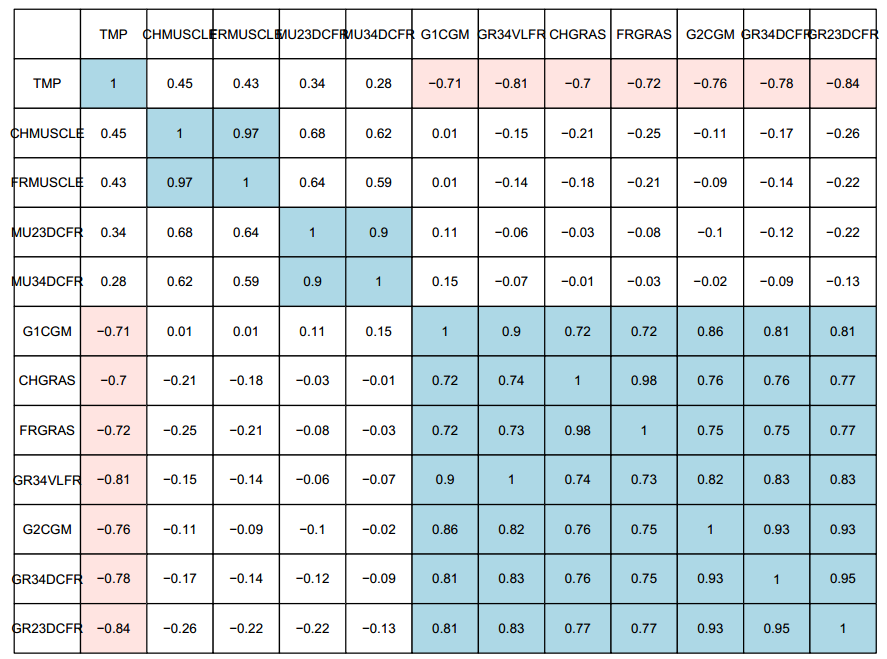
\includegraphics{Regression/Tableau-Correlation.png}
  \caption{Corrélations entre variables du jeu de données}
\end{figure}

\begin{Shaded}
\begin{Highlighting}[]
\NormalTok{mod}\OtherTok{\textless{}{-}}\FunctionTok{glm}\NormalTok{(TMP89}\SpecialCharTok{\textasciitilde{}}\NormalTok{.,}\AttributeTok{data=}\NormalTok{TMP[}\FunctionTok{is.na}\NormalTok{(TMP}\SpecialCharTok{$}\NormalTok{TMP89)}\SpecialCharTok{==}\NormalTok{F,}\FunctionTok{c}\NormalTok{(}\DecValTok{1}\NormalTok{,}\DecValTok{3}\SpecialCharTok{:}\DecValTok{41}\NormalTok{)])}
\FunctionTok{summary}\NormalTok{(mod)}
\end{Highlighting}
\end{Shaded}

\begin{verbatim}
% 
% Call:
% glm(formula = TMP89 ~ ., data = TMP[is.na(TMP$TMP89) == F, c(1, 
%     3:41)])
% 
% Coefficients: (6 not defined because of singularities)
%               Estimate Std. Error t value Pr(>|t|)
% (Intercept)  2.159e-12        NaN     NaN      NaN
% NUMORD      -1.039e-14        NaN     NaN      NaN
% ABATT1       3.537e-12        NaN     NaN      NaN
% CC           4.846e-14        NaN     NaN      NaN
% GGENE1       2.737e-13        NaN     NaN      NaN
% GGENE2      -1.475e-13        NaN     NaN      NaN
% GGENE3       9.109e-14        NaN     NaN      NaN
% SEXECH1      1.666e-13        NaN     NaN      NaN
% CHGRAS       5.999e-14        NaN     NaN      NaN
% CHMUSCLE     5.082e-14        NaN     NaN      NaN
% SEXCGM1             NA         NA      NA       NA
% G1CGM       -1.536e-14        NaN     NaN      NaN
% G2CGM       -1.407e-14        NaN     NaN      NaN
% M2CGM       -9.701e-15        NaN     NaN      NaN
% DATEFR1      3.572e-13        NaN     NaN      NaN
% DATEFR2     -5.723e-12        NaN     NaN      NaN
% DATEFR3      3.517e-13        NaN     NaN      NaN
% DATEFR4     -5.199e-12        NaN     NaN      NaN
% DATEFR5      3.458e-13        NaN     NaN      NaN
% DATEFR6     -5.124e-12        NaN     NaN      NaN
% DATEFR7      8.271e-13        NaN     NaN      NaN
% DATEFR8      4.116e-12        NaN     NaN      NaN
% DATEFR9     -4.643e-13        NaN     NaN      NaN
% DATEFR10     3.926e-12        NaN     NaN      NaN
% DATEFR11     4.303e-12        NaN     NaN      NaN
% DATEFR12     6.480e-13        NaN     NaN      NaN
% DATEFR13    -4.916e-12        NaN     NaN      NaN
% DATEFR14     1.234e-12        NaN     NaN      NaN
% DATEFR15    -4.569e-12        NaN     NaN      NaN
% DATEFR16     1.049e-12        NaN     NaN      NaN
% DATEFR17    -4.050e-12        NaN     NaN      NaN
% DATEFR18     8.797e-13        NaN     NaN      NaN
% DATEFR19     3.506e-12        NaN     NaN      NaN
% DATEFR20     3.440e-12        NaN     NaN      NaN
% DATEFR21     3.105e-12        NaN     NaN      NaN
% DATEFR22    -8.418e-13        NaN     NaN      NaN
% DATEFR23     3.465e-12        NaN     NaN      NaN
% DATEFR24    -4.167e-13        NaN     NaN      NaN
% DATEFR25            NA         NA      NA       NA
% SEXE1       -2.106e-13        NaN     NaN      NaN
% FRGRAS      -4.851e-14        NaN     NaN      NaN
% FRMUSCLE    -5.886e-14        NaN     NaN      NaN
% GR34VLFR    -3.358e-14        NaN     NaN      NaN
% GR23DCFR     1.750e-14        NaN     NaN      NaN
% GR34DCFR     9.918e-14        NaN     NaN      NaN
% GR34DCPAFR  -9.860e-14        NaN     NaN      NaN
% MU23DCFR     2.549e-14        NaN     NaN      NaN
% MU34DCFR     2.132e-14        NaN     NaN      NaN
% MU34DCPAFR  -4.050e-14        NaN     NaN      NaN
% FILPIECE    -5.401e-16        NaN     NaN      NaN
% LONPIECE     4.321e-15        NaN     NaN      NaN
% LONGEX      -4.399e-15        NaN     NaN      NaN
% EPAPIECE    -3.359e-15        NaN     NaN      NaN
% EPAGEX       3.728e-15        NaN     NaN      NaN
% JAMPIECE    -1.397e-15        NaN     NaN      NaN
% JAMGEX       1.381e-15        NaN     NaN      NaN
% LONMUGIOS   -4.189e-15        NaN     NaN      NaN
% EPAMUGIOS    2.988e-15        NaN     NaN      NaN
% JAMMUGIOS    1.191e-15        NaN     NaN      NaN
% LONPERTPAR          NA         NA      NA       NA
% EPAPERTPAR          NA         NA      NA       NA
% JAMPERTPAR          NA         NA      NA       NA
% TMUS3P      -1.710e-14        NaN     NaN      NaN
% TMP90        9.889e-01        NaN     NaN      NaN
% TVM         -2.391e-14        NaN     NaN      NaN
% DEN                 NA         NA      NA       NA
% 
% (Dispersion parameter for gaussian family taken to be NaN)
% 
%     Null deviance: 7.0543e+02  on 59  degrees of freedom
% Residual deviance: 8.6030e-26  on  0  degrees of freedom
% AIC: -3416.3
% 
% Number of Fisher Scoring iterations: 1
\end{verbatim}

\hypertarget{rstudio}{%
\section{Rstudio}\label{rstudio}}

\hypertarget{quelques-raccourcies}{%
\subsection{quelques raccourcies}\label{quelques-raccourcies}}

\hypertarget{rstudio-1}{%
\subsection{Rstudio}\label{rstudio-1}}

Quelques raccourcis intéressants : - \emph{ALT + -} : écrit de lisgne
d'assignation \textbf{\textless-} - \emph{CTRL + MAJ + M} écrira le
signe du pipe \textbf{\%\textgreater\%} - \emph{CTRL + MAJ + R} vous
permettra d'écrire proprement un titre de nouvelle section - \emph{CTRL
+ ALT + I} insérera un code chunk R dans votre code Rmarkdown -
\emph{CTRL + ALT + X} : alors celui-là est très intéressant. Si vous
avez un bout de code que vous souhaitez transformer en fonction, ce
raccourci-clavier fera tout le boulot tout seul, jusqu'à deviner le nom
des paramètres de la fonction, vous n'aurez qu'à entrer le nom de la
fonction. - \emph{ALT + L} réduit la section dans laquelle est le
curseur - \emph{ALT + MAJ + L} ouvre la section - \emph{ALT + O} réduit
toutes les sections - \emph{ALT + MAJ + O} ouvre toutes les sections -
\emph{CTRL + I} indente correctement le code sélectionné - \emph{CTRL +
MAJ + C} commente ou dé-commente la ligne active ou les ligne

Fonction cut -\textgreater{} Permet de transformet une quanti en quali
avec des intervalles données

Fonction smartbind de chez gtools -\textgreater{} faire du rbind avec
des colonnes mal agencées, permet du rbind selon le nom des colonnes.

Fonction droplevels -\textgreater{} Fait disparaître les niveaux de
facteurs non utilisés.

\pagebreak

\hypertarget{bibliographie}{%
\section*{Bibliographie}\label{bibliographie}}
\addcontentsline{toc}{section}{Bibliographie}

\hypertarget{refs}{}
\begin{CSLReferences}{1}{0}
\leavevmode\hypertarget{ref-hutton_number_2000}{}%
Hutton, J.L., 2000. Number {Needed} to {Treat}: {Properties} and
{Problems}. Journal of the Royal Statistical Society. Series A
(Statistics in Society) 163, 403--419.

\end{CSLReferences}

\end{document}
